
\documentclass[a4paper, 11pt, oneside]{book}

\usepackage{fontspec}
\usepackage[italian]{babel}
\usepackage{amsmath}
\usepackage{amssymb}
\usepackage{XCharter}
\usepackage[xcharter]{newtxmath}
\defaultfontfeatures{}
\setmonofont{JetBrainsMono Nerd Font}[
    Scale=MatchLowercase,
    Contextuals=NoAlternate % niente legature: -> resta -> come nel codice
]

\usepackage[a4paper, margin=2cm, headsep=10pt]{geometry}
\setlength{\headheight}{14pt}
\setlength{\emergencystretch}{1.5em}
\setcounter{tocdepth}{2}

\usepackage{fancyhdr}
\usepackage{float}
\usepackage{graphicx}
\usepackage{tabularx}
\usepackage{booktabs}
\usepackage[most]{tcolorbox}
\tcbuselibrary{skins, breakable, listings, theorems}
\usepackage{tikz}
\usetikzlibrary{fit, backgrounds, arrows.meta, calc, shapes.geometric}
\usepackage{fontawesome5}
% Ciclo di vita di una transazione Bitcoin, disegnato in TikZ.
% Caricato nel preambolo; definisce il comando
%   \ciclovita{<fase da evidenziare: 1-4, 0 = nessuna>}{<testo della nota, vuoto = nessuna nota>}
\definecolor{cvevidenza}{HTML}{C00000}
\definecolor{cvnota}{HTML}{E7E6E6}
\definecolor{cvnotabordo}{HTML}{7F7F7F}

\newcommand{\ciclovita}[2]{%
\scalebox{0.85}{% dimensione della figura
\begin{tikzpicture}[
    icona/.style={font=\fontsize{30}{30}\selectfont},
    intestazione/.style={font=\Large},
    numero/.style={fill=black, text=white, font=\Large, minimum width=0.75cm,
        minimum height=0.95cm, inner sep=0pt},
    fase/.style={align=left, font=\large, anchor=west, inner sep=2pt},
    freccia/.style={-{Triangle[length=5mm, width=6mm]}, line width=2.5pt}
]
    % attori
    \node[icona]        at (1.2, 5.2)  {\faUser};
    \node[intestazione] at (2.9, 5.2)  {Alice};
    \node[icona]        at (1.2, 3.9)  {\faCoins};
    \node[icona]        at (2.9, 3.9)  {\faSignature};
    \node[intestazione] at (8.3, 5.2)  {Network};
    % rete peer-to-peer: nodi collegati fra loro
    \begin{scope}[shift={(8.3, 3.95)}]
        \coordinate (r1) at (-0.65, 0.05);
        \coordinate (r2) at (-0.1, 0.5);
        \coordinate (r3) at (0.6, 0.35);
        \coordinate (r4) at (0.35, -0.4);
        \coordinate (r5) at (-0.35, -0.5);
        \draw[line width=1.6pt] (r1) -- (r2) -- (r3) -- (r4) -- (r5) -- (r1)
            (r2) -- (r4) (r1) -- (r4);
        \foreach \r in {r1, r2, r3, r4, r5}
            \fill (\r) circle (0.16);
    \end{scope}
    \node[intestazione] at (14.4, 5.2) {Blockchain};
    \node[icona]        at (14.4, 3.9) {\faCubes};
    \draw[freccia] (4.4, 4.2) -- (6.4, 4.2);
    \draw[freccia] (10.2, 4.2) -- (12.2, 4.2);

    % fasi
    \node[numero] (n1) at (0.4, 2.4)  {1};
    \node[fase]   (f1) at (0.9, 2.4)  {Creazione e firma\\della transazione};
    \node[numero] (n2) at (6.2, 2.4)  {2};
    \node[fase]   (f2) at (6.7, 2.4)  {Broadcast e validazione\\della transazione};
    \node[numero] (n3) at (12.3, 2.4) {3};
    \node[fase]   (f3) at (12.8, 2.4) {Mining o creazione\\dei blocchi};
    \draw[freccia] (14.4, 1.6) -- (14.4, 0.35);
    \node[icona]       at (14.4, -0.4) {\faCubes};
    \node[numero] (n4) at (10.2, -0.4) {4};
    \node[fase]   (f4) at (10.7, -0.4) {Transazione\\confermata};

    % fase evidenziata
    \ifnum#1>0
        \node[draw=cvevidenza, line width=1.3pt, inner sep=5pt, fit=(n#1)(f#1)] {};
    \fi

    % nota
    \if\relax\detokenize{#2}\relax\else
        \node[draw=cvnotabordo, fill=cvnota, anchor=west, text width=7.6cm,
            align=left, font=\large, inner sep=6pt] at (0, -0.4) {#2};
    \fi
\end{tikzpicture}}%
}
 % definisce \ciclovita
\usepackage[hidelinks]{hyperref} % caricato per ultimo

\pagestyle{fancy}
\fancyhf{}
\makeatletter
% numero del capitolo solo nel corpo principale, non nelle pagine degli indici
\renewcommand{\chaptermark}[1]{\markboth{\if@mainmatter\thechapter\quad\fi#1}{}}
\makeatother
\fancyhead[L]{\small\color{gray}\textsc{\nouppercase{\leftmark}}}
\fancyhead[R]{\small\thepage}
\renewcommand{\headrulewidth}{0.4pt}
\renewcommand{\headrule}{{\color{gray!40}\hrule height\headrulewidth width\headwidth}}

% codice
\definecolor{codeborder}{HTML}{505050}
\definecolor{codeback}{HTML}{F0F0F0}
\definecolor{codetitle}{HTML}{333333}
\definecolor{codekeyword}{HTML}{1F3FA8}
\definecolor{codetype}{HTML}{0E7C86}
\definecolor{codecomment}{HTML}{6A737D}
\definecolor{codestring}{HTML}{A31515}
% riquadri
\definecolor{defframe}{HTML}{1F3FA8}   % definizioni: blu
\definecolor{defback}{HTML}{EEF2FB}
\definecolor{noteframe}{HTML}{B7791F}  % note: ambra
\definecolor{noteback}{HTML}{FDF7E7}
\definecolor{warnframe}{HTML}{B42318}  % attenzione: rosso
\definecolor{warnback}{HTML}{FDEEEC}
\definecolor{exframe}{HTML}{1E7B45}    % esempi: verde
\definecolor{exback}{HTML}{ECF6EF}

\tcbset{
    riquadro/.style 2 args={
        breakable,
        enhanced,
        sharp corners,
        boxrule=0pt,
        leftrule=3pt,
        colframe=#1,
        colback=#2,
        fonttitle=\bfseries,
        coltitle=#1,
        attach title to upper={\ },
        before skip=10pt,
        after skip=10pt,
        boxsep=4pt,
        left=6pt,
        right=4pt
    }
}

\newtcbtheorem[number within=chapter]{definizione}{Definizione}{
    breakable,
    enhanced,
    sharp corners,
    boxrule=0.6pt,
    colframe=defframe,
    colback=defback,
    colbacktitle=defframe,
    coltitle=white,
    fonttitle=\bfseries,
    separator sign dash,
    before skip=10pt,
    after skip=10pt,
    boxsep=4pt,
    left=4pt,
    right=4pt
}{def}

% \begin{nota} ... \end{nota}  oppure  \begin{nota}[Titolo] ... \end{nota}
\newtcolorbox{nota}[1][Nota]{riquadro={noteframe}{noteback}, title={#1.}}
\newtcolorbox{attenzione}[1][Attenzione]{riquadro={warnframe}{warnback}, title={#1.}}
\newtcolorbox{esempio}[1][Esempio]{riquadro={exframe}{exback}, title={#1.}}

\lstdefinelanguage{Solidity}{
    morekeywords={pragma, solidity, contract, interface, library, abstract,
        function, modifier, event, emit, error, struct, enum, mapping, returns,
        return, public, private, internal, external, view, pure, payable,
        constant, immutable, memory, storage, calldata, if, else, for, while,
        do, break, continue, new, delete, import, is, using, override, virtual,
        constructor, receive, fallback, try, catch, unchecked, indexed,
        anonymous, require, revert, assert, true, false},
    morekeywords=[2]{address, bool, string, bytes, bytes4, bytes32, uint,
        uint8, uint16, uint32, uint64, uint128, uint256, int, int8, int256},
    sensitive=true,
    morecomment=[l]{//},
    morecomment=[s]{/*}{*/},
    morestring=[b]",
    morestring=[b]'
}

\DeclareTCBListing{codice}{ O{Codice} O{C} }{
    breakable,
    enhanced,
    sharp corners,
    boxrule=0.6pt,
    colframe=codeborder,
    colback=codeback,
    title={#1},
    fonttitle=\bfseries,
    coltitle=codetitle,
    attach title to upper={\par\smallskip},
    before skip=10pt,
    after skip=10pt,
    boxsep=4pt,
    left=4pt,
    right=4pt,
    listing only,
    listing options={
        language=#2,
        basicstyle=\ttfamily\footnotesize,
        keywordstyle=\color{codekeyword}\bfseries,
        keywordstyle={[2]\color{codetype}},
        commentstyle=\color{codecomment}\itshape,
        stringstyle=\color{codestring},
        showstringspaces=false,
        breaklines=true,
        tabsize=4,
        columns=fullflexible,
        keepspaces=true
    }
}

\newtcblisting{terminale}[1][Terminale]{
    breakable,
    enhanced,
    sharp corners,
    boxrule=0.6pt,
    colframe=codeborder,
    colback=white,
    title={#1},
    fonttitle=\bfseries,
    coltitle=codetitle,
    attach title to upper={\par\smallskip},
    before skip=10pt,
    after skip=10pt,
    boxsep=4pt,
    left=4pt,
    right=4pt,
    listing only,
    listing options={
        basicstyle=\ttfamily\footnotesize,
        breaklines=true,
        columns=fullflexible,
        keepspaces=true
    }
}

\newcommand{\cod}[1]{\texttt{#1}} % codice nel testo

\title{Introduzione alla programmazione di smart contract per Ethereum}
\author{Michele Castenedoli - VR519112}
\date{19 Novembre 2026}

\begin{document}
	\frontmatter
	\maketitle
	\tableofcontents

	\mainmatter
	\chapter{Lezione 01}
	\section{Cos'è una blockchain}
	Supponiamo di voler creare un consorzio per scambiare beni e servizi. Per gestire
	un'infrastruttura di questo tipo serve un \textbf{registro} (o libro contabile) in
	cui vengono memorizzati tutti gli scambi effettuati tra i partecipanti.

	Ogni voce del registro prende il nome di \textbf{transazione} e contiene le
	informazioni sullo scambio:
	\begin{itemize}
		\item chi offre il bene o il servizio;
		\item chi ne usufruisce;
		\item quando è avvenuta la transazione;
		\item il bene o il servizio fornito;
		\item la quantità scambiata.
	\end{itemize}

	Il primo problema deriva dalla natura del consorzio, che è un ambiente distribuito:
	chi tiene il registro? La soluzione tradizionale consiste nell'eleggere un'entità
	terza che mantiene il registro e di cui tutti si fidano. Questa soluzione, però,
	funziona solo se il consorzio è ristretto e non ci sono problemi di fiducia tra i
	membri; inoltre resta aperta la domanda su chi debba scegliere l'entità terza.

	Una \textbf{blockchain} elimina il problema alla radice: ogni membro del consorzio
	mantiene una copia del registro. Bisogna allora garantire che tutte le copie
	coincidano, e per questo si usa un protocollo di consenso decentralizzato, cioè un
	insieme di regole di natura informatica, giuridica ed economica. L'obiettivo è
	prevedere penalità così elevate da rendere non conveniente mentire nella scrittura
	del registro: tutti sono incentivati a comportarsi in modo onesto. Il meccanismo
	prende forme diverse a seconda che si usi la \textit{Proof of Work} o la
	\textit{Proof of Stake}.

	La grande innovazione della blockchain è quindi la possibilità di lavorare in un
	ambiente distribuito e decentralizzato, in cui sono regole informatiche ed
	economiche a obbligare tutti i membri a comportarsi in modo lecito.

	La blockchain è inoltre \textbf{immutabile}: le transazioni vengono registrate in
	gruppi chiamati \textbf{blocchi} e, una volta scritto un blocco, il suo contenuto
	non può più essere modificato.

	\section{Bitcoin e Blockchain}
	Prima di Bitcoin c'erano stati diversi tentativi, ma è con questa criptovaluta e
	con l'avvento della blockchain che si è arrivati a definire un protocollo per
	costruire una rete \textit{peer-to-peer}\footnote{Una rete in cui tutti i nodi sono
	``alla pari''.} in grado di raggiungere il consenso su uno stato globale senza
	l'intervento di un'entità centrale.

	In particolare, la blockchain è stata usata inizialmente per risolvere il problema
	del \textit{double spending} senza ricorrere a un'entità centrale. Un'autorità
	centrale è anzi essa stessa un problema: richiede la fiducia di tutti i
	partecipanti e rappresenta un possibile punto di partenza per attaccare l'intera
	infrastruttura.

	\begin{definizione}{Transazione}{transaction}
		Una \textbf{transazione} è una struttura dati che descrive il trasferimento di
		una certa quantità di token da uno o più indirizzi di partenza (\textit{input})
		a uno o più indirizzi di destinazione (\textit{output}).
	\end{definizione}

	Proseguendo l'analogia con il registro, una pagina di transazioni prende il nome
	di \textbf{blocco}. Ogni blocco è concatenato al precedente, quindi non è possibile
	modificare un blocco senza modificare anche tutti quelli successivi.

	\begin{definizione}{Bitcoin}{bitcoin}
		Bitcoin è un automa per il consenso distribuito, in cui:
		\begin{enumerate}
			\item le transizioni da uno stato all'altro sono le transazioni
				(definizione~\ref{def:transaction});
			\item gli stati sono corrispondenze del tipo
				\cod{indirizzo} $\rightarrow$ \cod{numero di token}.
		\end{enumerate}
	\end{definizione}

	\section{Ciclo di vita di una transazione Bitcoin}
	Una transazione Bitcoin attraversa quattro fasi:
	\begin{enumerate}
		\item \textbf{creazione e firma}: Alice crea la transazione con il proprio wallet
			e la firma;
		\item \textbf{broadcast e validazione}: la transazione viene inviata alla rete, i
			cui nodi la controllano e la diffondono;
		\item \textbf{mining}: la transazione viene inserita in un nuovo blocco;
		\item \textbf{conferma}: il blocco entra a far parte della blockchain e la
			transazione è confermata.
	\end{enumerate}
	Le sezioni seguenti descrivono le fasi una per una.

	\section{Fase 1: creazione e firma della transazione}
	\begin{figure}[H]
		\centering
		\ciclovita{1}{Tramite la firma si prova il possesso dei token e si autorizza a
			spenderli}
		\caption{Prima fase: creazione e firma della transazione.}
		\label{fig:ciclo-vita-fase1}
	\end{figure}

	Nella prima fase Alice crea la transazione tramite il proprio \textit{wallet}
	(definizione~\ref{def:wallet}) e la autorizza con la \textbf{firma}, che attesta che
	è lei la proprietaria dei token.

	\subsection{Wallet e chiavi}
	\begin{definizione}{Wallet}{wallet}
		Un \textbf{wallet} è un'applicazione software che fa da interfaccia principale tra
		l'utente e una blockchain. Il suo compito è raccogliere i dati di una transazione,
		codificarli nell'apposita struttura dati e firmare la transazione.
	\end{definizione}

	Le firme si basano su una coppia di chiavi, una pubblica e una privata. La chiave
	privata, con cui si firma, deve restare segreta. Dalla chiave pubblica si ricava
	l'\textbf{indirizzo}, che è ciò che si comunica agli altri per ricevere token. La
	chiave pubblica diventa visibile solo quando si spendono i token: viene inserita
	nella transazione per permettere ai nodi di verificare la firma.

	Indirizzi e transazioni sono pubblici: tutte le transazioni sono registrate sulla
	blockchain e chiunque può leggerle. A differenza di un'app di home banking, quindi,
	un wallet non conserva i saldi ma le chiavi pubbliche e private; il saldo che mostra
	viene calcolato leggendo la blockchain.

	\subsection{Generazione delle chiavi}
	Quando un wallet viene avviato per la prima volta:
	\begin{enumerate}
		\item genera, con un generatore di numeri casuali sicuro, una sequenza finita di
			bit: è la \textbf{chiave privata}, che deve restare segreta;
		\item dalla chiave privata calcola la chiave pubblica e da questa, con una funzione
			di \textit{hash}, l'\textbf{indirizzo};
		\item mostra l'indirizzo come stringa alfanumerica oppure come codice QR.
	\end{enumerate}

	\begin{nota}
		Qui non basta un generatore pseudocasuale di libreria: serve vera entropia,
		raccolta per esempio dallo stato del dispositivo, dai movimenti del cursore o dalle
		variazioni di temperatura. I numeri devono essere davvero imprevedibili.
	\end{nota}

	L'indirizzo non è un'informazione sensibile: Alice può pubblicarlo, per esempio sulla
	propria pagina web.

	\begin{attenzione}
		La chiave privata è un'informazione sensibile e Alice deve mantenerla segreta.
		Il rischio dipende da dove il wallet la conserva; in ordine di rischio crescente:
		\begin{itemize}
			\item \textbf{wallet hardware}: nella propria memoria, da cui la chiave non esce
				mai;
			\item \textbf{wallet desktop}: nel computer;
			\item \textbf{wallet mobile}: nel telefono;
			\item \textbf{wallet web}: nel cloud oppure sul server di terze parti.
		\end{itemize}
	\end{attenzione}
	A seconda del wallet utilizzato, quindi, cambia il livello di sicurezza.

	\subsection{Wallet deterministici}
	In base a come generano le chiavi, i wallet si dividono in due tipi:
	\begin{itemize}
		\item \textbf{non deterministici}: ogni chiave è indipendente dalle altre e viene
			generata a partire da un numero casuale diverso per ogni chiave;
		\item \textbf{deterministici}: tutte le chiavi derivano da un unico valore iniziale,
			il \textbf{seed} (o \textit{master key}).
			Conoscendo il seed originale si possono rigenerare tutte le chiavi. La forma
			più evoluta è il \textbf{wallet deterministico gerarchico}, definito dallo
			standard BIP-32.
	\end{itemize}

	Un wallet deterministico gerarchico, come MetaMask, contiene una serie di chiavi
	derivate secondo una struttura ad albero (figura~\ref{fig:wallet-gerarchico}): dal
	seed si ottiene la master key $k_m$, da questa le chiavi figlie ($k_m/0$, $k_m/1$,
	\dots) e da ciascuna figlia le chiavi nipoti. Inoltre è possibile creare una
	sequenza di chiavi pubbliche senza dare accesso alle chiavi private corrispondenti.

	\begin{figure}[H]
		\centering
		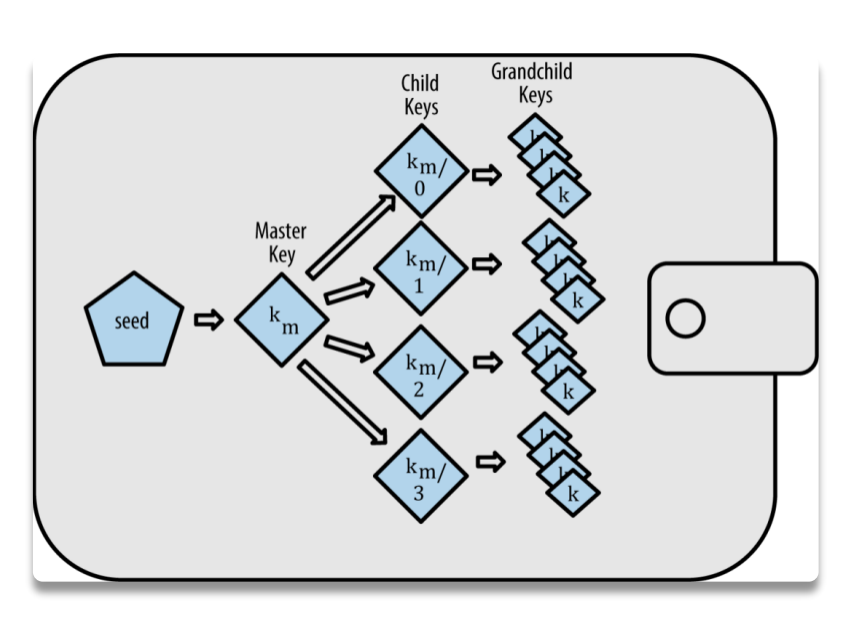
\includegraphics[width=0.4\textwidth]{immagini/wallet-gerarchico.png}
		\caption{Derivazione delle chiavi in un wallet deterministico gerarchico.}
		\label{fig:wallet-gerarchico}
	\end{figure}

	\subsection{Codice mnemonico}
	Il seed di un wallet deterministico si ricava da un \textbf{codice mnemonico}, cioè
	una sequenza di 12 parole definita dallo standard BIP-39. Il codice si genera così
	(figura~\ref{fig:parole-mnemoniche}):
	\begin{enumerate}
		\item si generano 128 bit di entropia con un generatore di numeri casuali sicuro;
		\item si calcola lo SHA-256 dell'entropia e se ne prendono i primi 4 bit, che
			fanno da \textit{checksum};
		\item si accodano i 4 bit di checksum ai 128 bit di entropia, ottenendo 132 bit;
		\item si dividono i 132 bit in 12 blocchi da 11 bit ciascuno;
		\item ogni blocco è un numero da 0 a 2047 e indica una parola in una lista
			standard di 2048 parole;
		\item le 12 parole ottenute formano il codice mnemonico.
	\end{enumerate}
	Con 256 bit di entropia il procedimento è lo stesso: il checksum è di 8 bit e si
	ottengono 24 parole.

	\begin{figure}[H]
		\centering
		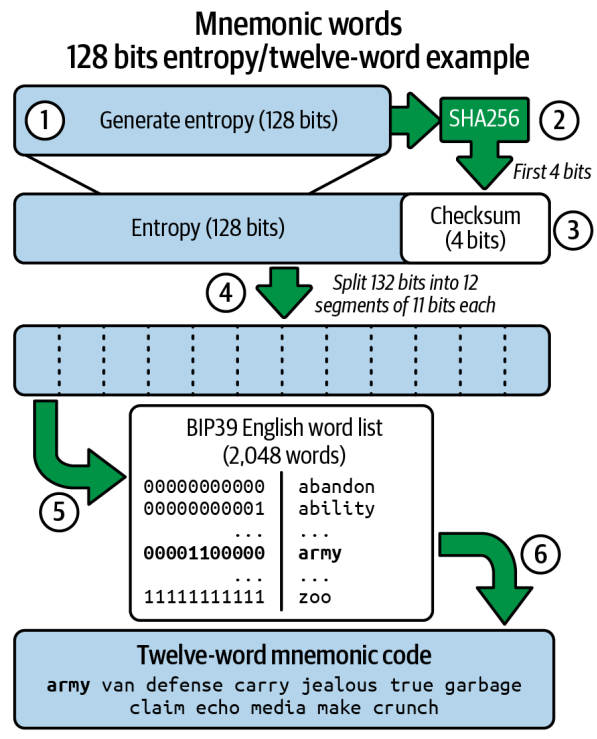
\includegraphics[width=0.45\textwidth]{immagini/parole-mnemoniche.png}
		\caption{Generazione di un codice mnemonico di 12 parole (BIP-39).}
		\label{fig:parole-mnemoniche}
	\end{figure}

	Le parole contengono la stessa informazione dell'entropia, ma in una forma che una
	persona può trascrivere facilmente. Il checksum serve ad accorgersi degli errori di
	trascrizione: una parola sbagliata o un ordine sbagliato rendono quasi sempre il
	codice non valido.

	Dal codice mnemonico si ricavano tutte le chiavi del wallet con algoritmi standard e
	deterministici:
	\begin{enumerate}
		\item le parole, insieme a una password facoltativa, passano nella funzione
			PBKDF2-HMAC-SHA512 con 2048 iterazioni, fissate dallo standard, che produce
			un seed di 512 bit;
		\item dal seed si ottiene la master key privata e da questa le chiavi private
			figlie, nipoti e così via (BIP-32);
		\item da ogni chiave privata si calcola la chiave pubblica e da questa
			l'indirizzo.
	\end{enumerate}
	Le stesse parole, con la stessa password, producono sempre le stesse chiavi: per
	recuperare il wallet, anche su un altro dispositivo, basta reinserirle.

	\begin{attenzione}
		Il codice mnemonico è il backup dell'intero wallet: chi conosce le parole
		controlla tutti i fondi. Va conservato offline, per esempio scritto su carta.
	\end{attenzione}

	\subsection{Unspent Transaction Output (UTXO)}
	\begin{definizione}{Unspent Transaction Output}{utxo}
		In Bitcoin un \textbf{UTXO} (\textit{Unspent Transaction Output}) è un insieme di
		token attualmente assegnati a un indirizzo e non ancora spesi.
	\end{definizione}

	Ogni transazione consuma alcuni UTXO e ne crea di nuovi:
	\begin{itemize}
		\item gli \textbf{input} di una transazione sono gli UTXO che la transazione
			consuma;
		\item gli \textbf{output} di una transazione sono gli UTXO che la transazione crea.
	\end{itemize}
	L'insieme degli UTXO è una parte fondamentale dello \textbf{stato globale} della
	blockchain di Bitcoin: associa a ogni indirizzo i token che possiede
	(definizione~\ref{def:bitcoin}). Il saldo di un indirizzo è quindi la somma degli
	UTXO che gli sono assegnati.

	Gli output di una transazione sono numerati a partire da 0. Un input indica l'UTXO
	che spende tramite l'identificativo della transazione che lo ha creato, seguito
	dal numero dell'output: per esempio \cod{7957a3...f6f18:0} è l'output numero 0 della
	transazione \cod{7957a3...f6f18}. Il numero indica solo la posizione dell'output e
	non dice quale output va al destinatario.

	Un UTXO si spende sempre per intero. Se vale più della somma da trasferire, la
	transazione contiene un output in più che riporta la differenza a un indirizzo del
	mittente: è il \textbf{resto} (\textit{change}), che diventa a sua volta un nuovo
	UTXO del mittente.

	Poiché ogni input fa riferimento a un output di una transazione precedente, le
	transazioni formano un \textbf{grafo aciclico}. Nella
	figura~\ref{fig:grafo-transazioni} Joe trasferisce 0.1 BTC ad Alice; Alice spende
	quell'UTXO per intero, inviando 0.015 BTC a Bob e riportando il resto a sé stessa;
	Bob spende a sua volta l'UTXO ricevuto, inviando 0.01 BTC a Gopesh e tenendo il
	resto. Gli output segnati come \textit{spent} sono già stati usati come input di
	un'altra transazione, quelli \textit{unspent} sono gli UTXO ancora disponibili.

	\begin{figure}[H]
		\centering
		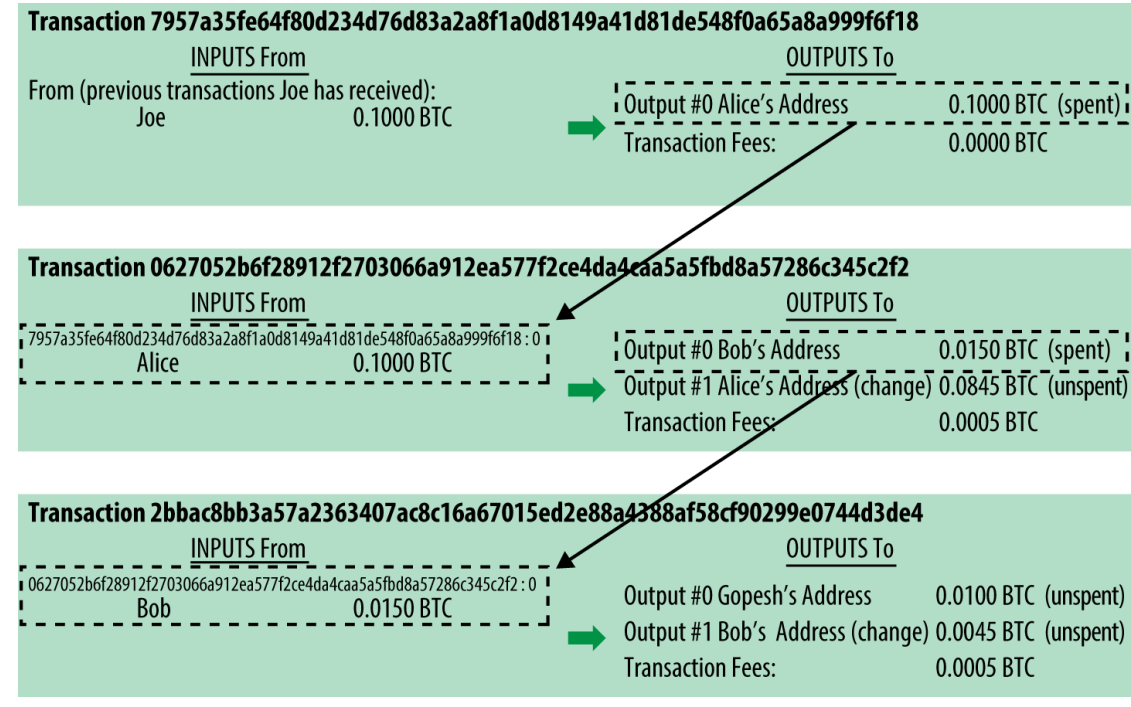
\includegraphics[width=0.8\textwidth]{immagini/grafo-transazioni.png}
		\caption{Grafo aciclico di transazioni.}
		\label{fig:grafo-transazioni}
	\end{figure}

	L'esempio della figura~\ref{fig:grafo-transazioni} è una semplice catena, ma in
	generale una transazione può avere più input, provenienti da transazioni diverse, e
	più output, spesi da transazioni diverse: il grafo può quindi sia diramarsi sia
	ricongiungersi (figura~\ref{fig:dag-transazioni}). È aciclico perché un input può
	fare riferimento solo a un output già esistente. Nella figura le frecce continue
	sono output già spesi, quelle tratteggiate gli UTXO ancora disponibili; i valori
	sono in migliaia di satoshi (kS), dove 1 satoshi vale 0.00000001 BTC.

	\begin{figure}[H]
		\centering
		% Grafo di transazioni con diramazioni e confluenze (valori in migliaia di satoshi).
% Incluso nel documento con % Grafo di transazioni con diramazioni e confluenze (valori in migliaia di satoshi).
% Incluso nel documento con % Grafo di transazioni con diramazioni e confluenze (valori in migliaia di satoshi).
% Incluso nel documento con \input{immagini/dag-transazioni.tex}.
\definecolor{dagtx}{HTML}{DAE3F3}
\definecolor{dagtxborder}{HTML}{4472C4}
\definecolor{dagin}{HTML}{E7E6E6}
\definecolor{daginborder}{HTML}{A6A6A6}
\definecolor{dagout}{HTML}{E2F0D9}
\definecolor{dagoutborder}{HTML}{70AD47}
\definecolor{dagval}{HTML}{FFF2CC}
\resizebox{\textwidth}{!}{%
\begin{tikzpicture}[
    port/.style={draw, minimum width=2.1cm, minimum height=0.62cm, font=\bfseries},
    ingresso/.style={port, fill=dagin, draw=daginborder},
    uscita/.style={port, fill=dagout, draw=dagoutborder},
    titolo/.style={font=\bfseries\large},
    tx/.style={draw=dagtxborder, fill=dagtx, inner sep=0.28cm},
    val/.style={draw, solid, line width=0.4pt, fill=dagval, rounded corners=2pt, font=\small, inner sep=2.5pt},
    txo/.style={-{Latex[length=2.6mm]}, line width=1.4pt},
    utxo/.style={txo, dotted, line width=1.8pt}
]
    % --- Tx0 ---
    \node[titolo] (t0)  at (0, 3.1) {Tx0};
    \node[ingresso]     (t0i0) at (0, 2.4) {input0};
    \node[uscita]    (t0o0) at (0, 1.6) {output0};
    \node[uscita]    (t0o1) at (0, 0.8) {output1};
    % --- Tx1 ---
    \node[titolo] (t1)  at (4.3, 5.0) {Tx1};
    \node[ingresso]     (t1i0) at (4.3, 4.3) {input0};
    \node[uscita]    (t1o0) at (4.3, 3.5) {output0};
    \node[uscita]    (t1o1) at (4.3, 2.7) {output1};
    % --- Tx2 ---
    \node[titolo] (t2)  at (4.3, 1.3) {Tx2};
    \node[ingresso]     (t2i0) at (4.3, 0.6) {input0};
    \node[uscita]    (t2o0) at (4.3, -0.2) {output0};
    % --- Tx3 ---
    \node[titolo] (t3)  at (8.6, 5.0) {Tx3};
    \node[ingresso]     (t3i0) at (8.6, 4.3) {input0};
    \node[ingresso]     (t3i1) at (8.6, 3.5) {input1};
    \node[uscita]    (t3o0) at (8.6, 2.7) {output0};
    % --- Tx4 ---
    \node[titolo] (t4)  at (8.6, 1.3) {Tx4};
    \node[ingresso]     (t4i0) at (8.6, 0.6) {input0};
    \node[uscita]    (t4o0) at (8.6, -0.2) {output0};
    \node[uscita]    (t4o1) at (8.6, -1.0) {output1};
    % --- Tx5 ---
    \node[titolo] (t5)  at (12.9, 3.6) {Tx5};
    \node[ingresso]     (t5i0) at (12.9, 2.9) {input0};
    \node[ingresso]     (t5i1) at (12.9, 2.1) {input1};
    \node[ingresso]     (t5i2) at (12.9, 1.3) {input2};
    \node[uscita]    (t5o0) at (12.9, 0.5) {output0};

    % riquadri delle transazioni, dietro alle porte
    \begin{scope}[on background layer]
        \node[tx, fit=(t0)(t0i0)(t0o1)] {};
        \node[tx, fit=(t1)(t1i0)(t1o1)] {};
        \node[tx, fit=(t2)(t2i0)(t2o0)] {};
        \node[tx, fit=(t3)(t3i0)(t3o0)] {};
        \node[tx, fit=(t4)(t4i0)(t4o1)] {};
        \node[tx, fit=(t5)(t5i0)(t5o0)] {};
    \end{scope}

    % output spesi (TXO)
    \draw[txo] (-2.9, 2.4) -- node[val] {150kS} (t0i0.west);
    \draw[txo] (t0o0.east) -- node[val] {50kS}  (t1i0.west);
    \draw[txo] (t0o1.east) -- node[val] {100kS} (t2i0.west);
    \draw[txo] (t1o0.east) -- node[val] {10kS}  (t3i0.west);
    \draw[txo] (t1o1.east) -- node[val] {40kS}  (t3i1.west);
    \draw[txo] (t2o0.east) -- node[val] {100kS} (t4i0.west);
    \draw[txo] (t3o0.east) -- node[val] {50kS}  (t5i0.west);
    \draw[txo] (t4o0.east) -- node[val] {30kS}  (t5i1.west);

    % output non spesi (UTXO)
    \draw[utxo] (t4o1.east) -- node[val] {70kS}  ++(2.9, 0);
    \draw[utxo] (t5o0.east) -- node[val] {150kS} ++(2.9, 0);

    % legenda
    \draw[utxo] (12.0, 5.75) -- ++(1.2, 0) node[right, font=\bfseries\small] {UTXO};
    \draw[txo]  (12.0, 5.25) -- ++(1.2, 0) node[right, font=\bfseries\small] {TXO};
    \node[val, anchor=west] at (12.0, 4.75) {valore in satoshi};
\end{tikzpicture}%
}
.
\definecolor{dagtx}{HTML}{DAE3F3}
\definecolor{dagtxborder}{HTML}{4472C4}
\definecolor{dagin}{HTML}{E7E6E6}
\definecolor{daginborder}{HTML}{A6A6A6}
\definecolor{dagout}{HTML}{E2F0D9}
\definecolor{dagoutborder}{HTML}{70AD47}
\definecolor{dagval}{HTML}{FFF2CC}
\resizebox{\textwidth}{!}{%
\begin{tikzpicture}[
    port/.style={draw, minimum width=2.1cm, minimum height=0.62cm, font=\bfseries},
    ingresso/.style={port, fill=dagin, draw=daginborder},
    uscita/.style={port, fill=dagout, draw=dagoutborder},
    titolo/.style={font=\bfseries\large},
    tx/.style={draw=dagtxborder, fill=dagtx, inner sep=0.28cm},
    val/.style={draw, solid, line width=0.4pt, fill=dagval, rounded corners=2pt, font=\small, inner sep=2.5pt},
    txo/.style={-{Latex[length=2.6mm]}, line width=1.4pt},
    utxo/.style={txo, dotted, line width=1.8pt}
]
    % --- Tx0 ---
    \node[titolo] (t0)  at (0, 3.1) {Tx0};
    \node[ingresso]     (t0i0) at (0, 2.4) {input0};
    \node[uscita]    (t0o0) at (0, 1.6) {output0};
    \node[uscita]    (t0o1) at (0, 0.8) {output1};
    % --- Tx1 ---
    \node[titolo] (t1)  at (4.3, 5.0) {Tx1};
    \node[ingresso]     (t1i0) at (4.3, 4.3) {input0};
    \node[uscita]    (t1o0) at (4.3, 3.5) {output0};
    \node[uscita]    (t1o1) at (4.3, 2.7) {output1};
    % --- Tx2 ---
    \node[titolo] (t2)  at (4.3, 1.3) {Tx2};
    \node[ingresso]     (t2i0) at (4.3, 0.6) {input0};
    \node[uscita]    (t2o0) at (4.3, -0.2) {output0};
    % --- Tx3 ---
    \node[titolo] (t3)  at (8.6, 5.0) {Tx3};
    \node[ingresso]     (t3i0) at (8.6, 4.3) {input0};
    \node[ingresso]     (t3i1) at (8.6, 3.5) {input1};
    \node[uscita]    (t3o0) at (8.6, 2.7) {output0};
    % --- Tx4 ---
    \node[titolo] (t4)  at (8.6, 1.3) {Tx4};
    \node[ingresso]     (t4i0) at (8.6, 0.6) {input0};
    \node[uscita]    (t4o0) at (8.6, -0.2) {output0};
    \node[uscita]    (t4o1) at (8.6, -1.0) {output1};
    % --- Tx5 ---
    \node[titolo] (t5)  at (12.9, 3.6) {Tx5};
    \node[ingresso]     (t5i0) at (12.9, 2.9) {input0};
    \node[ingresso]     (t5i1) at (12.9, 2.1) {input1};
    \node[ingresso]     (t5i2) at (12.9, 1.3) {input2};
    \node[uscita]    (t5o0) at (12.9, 0.5) {output0};

    % riquadri delle transazioni, dietro alle porte
    \begin{scope}[on background layer]
        \node[tx, fit=(t0)(t0i0)(t0o1)] {};
        \node[tx, fit=(t1)(t1i0)(t1o1)] {};
        \node[tx, fit=(t2)(t2i0)(t2o0)] {};
        \node[tx, fit=(t3)(t3i0)(t3o0)] {};
        \node[tx, fit=(t4)(t4i0)(t4o1)] {};
        \node[tx, fit=(t5)(t5i0)(t5o0)] {};
    \end{scope}

    % output spesi (TXO)
    \draw[txo] (-2.9, 2.4) -- node[val] {150kS} (t0i0.west);
    \draw[txo] (t0o0.east) -- node[val] {50kS}  (t1i0.west);
    \draw[txo] (t0o1.east) -- node[val] {100kS} (t2i0.west);
    \draw[txo] (t1o0.east) -- node[val] {10kS}  (t3i0.west);
    \draw[txo] (t1o1.east) -- node[val] {40kS}  (t3i1.west);
    \draw[txo] (t2o0.east) -- node[val] {100kS} (t4i0.west);
    \draw[txo] (t3o0.east) -- node[val] {50kS}  (t5i0.west);
    \draw[txo] (t4o0.east) -- node[val] {30kS}  (t5i1.west);

    % output non spesi (UTXO)
    \draw[utxo] (t4o1.east) -- node[val] {70kS}  ++(2.9, 0);
    \draw[utxo] (t5o0.east) -- node[val] {150kS} ++(2.9, 0);

    % legenda
    \draw[utxo] (12.0, 5.75) -- ++(1.2, 0) node[right, font=\bfseries\small] {UTXO};
    \draw[txo]  (12.0, 5.25) -- ++(1.2, 0) node[right, font=\bfseries\small] {TXO};
    \node[val, anchor=west] at (12.0, 4.75) {valore in satoshi};
\end{tikzpicture}%
}
.
\definecolor{dagtx}{HTML}{DAE3F3}
\definecolor{dagtxborder}{HTML}{4472C4}
\definecolor{dagin}{HTML}{E7E6E6}
\definecolor{daginborder}{HTML}{A6A6A6}
\definecolor{dagout}{HTML}{E2F0D9}
\definecolor{dagoutborder}{HTML}{70AD47}
\definecolor{dagval}{HTML}{FFF2CC}
\resizebox{\textwidth}{!}{%
\begin{tikzpicture}[
    port/.style={draw, minimum width=2.1cm, minimum height=0.62cm, font=\bfseries},
    ingresso/.style={port, fill=dagin, draw=daginborder},
    uscita/.style={port, fill=dagout, draw=dagoutborder},
    titolo/.style={font=\bfseries\large},
    tx/.style={draw=dagtxborder, fill=dagtx, inner sep=0.28cm},
    val/.style={draw, solid, line width=0.4pt, fill=dagval, rounded corners=2pt, font=\small, inner sep=2.5pt},
    txo/.style={-{Latex[length=2.6mm]}, line width=1.4pt},
    utxo/.style={txo, dotted, line width=1.8pt}
]
    % --- Tx0 ---
    \node[titolo] (t0)  at (0, 3.1) {Tx0};
    \node[ingresso]     (t0i0) at (0, 2.4) {input0};
    \node[uscita]    (t0o0) at (0, 1.6) {output0};
    \node[uscita]    (t0o1) at (0, 0.8) {output1};
    % --- Tx1 ---
    \node[titolo] (t1)  at (4.3, 5.0) {Tx1};
    \node[ingresso]     (t1i0) at (4.3, 4.3) {input0};
    \node[uscita]    (t1o0) at (4.3, 3.5) {output0};
    \node[uscita]    (t1o1) at (4.3, 2.7) {output1};
    % --- Tx2 ---
    \node[titolo] (t2)  at (4.3, 1.3) {Tx2};
    \node[ingresso]     (t2i0) at (4.3, 0.6) {input0};
    \node[uscita]    (t2o0) at (4.3, -0.2) {output0};
    % --- Tx3 ---
    \node[titolo] (t3)  at (8.6, 5.0) {Tx3};
    \node[ingresso]     (t3i0) at (8.6, 4.3) {input0};
    \node[ingresso]     (t3i1) at (8.6, 3.5) {input1};
    \node[uscita]    (t3o0) at (8.6, 2.7) {output0};
    % --- Tx4 ---
    \node[titolo] (t4)  at (8.6, 1.3) {Tx4};
    \node[ingresso]     (t4i0) at (8.6, 0.6) {input0};
    \node[uscita]    (t4o0) at (8.6, -0.2) {output0};
    \node[uscita]    (t4o1) at (8.6, -1.0) {output1};
    % --- Tx5 ---
    \node[titolo] (t5)  at (12.9, 3.6) {Tx5};
    \node[ingresso]     (t5i0) at (12.9, 2.9) {input0};
    \node[ingresso]     (t5i1) at (12.9, 2.1) {input1};
    \node[ingresso]     (t5i2) at (12.9, 1.3) {input2};
    \node[uscita]    (t5o0) at (12.9, 0.5) {output0};

    % riquadri delle transazioni, dietro alle porte
    \begin{scope}[on background layer]
        \node[tx, fit=(t0)(t0i0)(t0o1)] {};
        \node[tx, fit=(t1)(t1i0)(t1o1)] {};
        \node[tx, fit=(t2)(t2i0)(t2o0)] {};
        \node[tx, fit=(t3)(t3i0)(t3o0)] {};
        \node[tx, fit=(t4)(t4i0)(t4o1)] {};
        \node[tx, fit=(t5)(t5i0)(t5o0)] {};
    \end{scope}

    % output spesi (TXO)
    \draw[txo] (-2.9, 2.4) -- node[val] {150kS} (t0i0.west);
    \draw[txo] (t0o0.east) -- node[val] {50kS}  (t1i0.west);
    \draw[txo] (t0o1.east) -- node[val] {100kS} (t2i0.west);
    \draw[txo] (t1o0.east) -- node[val] {10kS}  (t3i0.west);
    \draw[txo] (t1o1.east) -- node[val] {40kS}  (t3i1.west);
    \draw[txo] (t2o0.east) -- node[val] {100kS} (t4i0.west);
    \draw[txo] (t3o0.east) -- node[val] {50kS}  (t5i0.west);
    \draw[txo] (t4o0.east) -- node[val] {30kS}  (t5i1.west);

    % output non spesi (UTXO)
    \draw[utxo] (t4o1.east) -- node[val] {70kS}  ++(2.9, 0);
    \draw[utxo] (t5o0.east) -- node[val] {150kS} ++(2.9, 0);

    % legenda
    \draw[utxo] (12.0, 5.75) -- ++(1.2, 0) node[right, font=\bfseries\small] {UTXO};
    \draw[txo]  (12.0, 5.25) -- ++(1.2, 0) node[right, font=\bfseries\small] {TXO};
    \node[val, anchor=west] at (12.0, 4.75) {valore in satoshi};
\end{tikzpicture}%
}

		\caption{Grafo di transazioni con diramazioni e confluenze.}
		\label{fig:dag-transazioni}
	\end{figure}

	\subsection{Come il wallet prepara la transazione}
	Per inviare token, il wallet di Alice costruisce la transazione in questo modo:
	\begin{enumerate}
		\item seleziona, tra gli UTXO a disposizione di Alice, un insieme da usare come
			\textbf{input}, in modo da avere un quantitativo sufficiente di token. Sono a
			disposizione di Alice gli UTXO associati a un indirizzo di cui lei possiede la
			chiave privata: il wallet ne mantiene una copia in cache e, se non ha
			informazioni sufficienti, li chiede alla rete;
		\item specifica come primo output l'indirizzo del destinatario e il quantitativo
			di token da inviargli, $\text{amount} \ge 0$;
		\item specifica come secondo output un indirizzo di Alice, che riceve il resto,
			$\text{change} \ge 0$.
	\end{enumerate}
	La differenza tra gli input e gli output è la \textbf{fee}, pagata per far processare
	la transazione e incassata dal miner che la inserisce in un blocco:
	\[
		\text{fee} = \sum \text{inputs} - \text{amount} - \text{change} \ge 0
	\]
	La fee non compare esplicitamente nella transazione. Per esempio, nella seconda
	transazione della figura~\ref{fig:grafo-transazioni} l'input vale 0.1000 BTC,
	l'amount 0.0150 BTC e il change 0.0845 BTC, quindi la fee è di 0.0005 BTC.

	\section{Fase 2: broadcast e validazione della transazione}
	\begin{figure}[H]
		\centering
		\ciclovita{2}{Ciascun nodo della rete riceve la nuova transazione, ne verifica
			la validità e, se è valida, la passa ai vicini}
		\caption{Seconda fase: broadcast e validazione della transazione.}
		\label{fig:ciclo-vita-fase2}
	\end{figure}

	Una volta firmata, la transazione viene inviata (\textit{broadcast}) alla rete
	\textit{peer-to-peer}. Ciascun nodo che la riceve la controlla, verificando per
	esempio la firma e che gli UTXO in input non siano già stati spesi, e se è valida
	la passa ai nodi vicini: in questo modo la transazione si propaga in tutta la rete.

	\section{Fase 3: mining o creazione dei blocchi}\label{sec:fase3-mining}
	\begin{figure}[H]
		\centering
		\ciclovita{3}{}
		\caption{Terza fase: mining o creazione dei blocchi.}
		\label{fig:ciclo-vita-fase3}
	\end{figure}

	I nodi che ricevono una transazione la conservano in un'area di memoria chiamata
	\textbf{mempool}, dove resta in attesa (\textit{pendente}) finché un miner non la
	inserisce in un blocco. La creazione di un nuovo blocco prende il nome di
	\textbf{mining}.

	Ciascun miner costruisce un blocco candidato che contiene:
	\begin{itemize}
		\item le transazioni che ha selezionato dalla mempool;
		\item una transazione speciale, la \textbf{coinbase}, che non consuma nessun UTXO
			e ha come output l'indirizzo del miner, con una quantità di token pari alla
			ricompensa per il blocco (\textit{mining reward}) più le fee delle transazioni
			incluse;
		\item l'hash del blocco precedente, che lo collega alla catena;
		\item un \textbf{nonce}, cioè un numero scelto in modo che l'hash del blocco inizi
			con un certo numero prefissato di zeri. Non c'è modo di calcolarlo
			direttamente: l'unico modo per trovarlo è provare valori diversi finché non se
			ne trova uno valido. È questo il lavoro richiesto dalla \textit{Proof of Work}.
			Più zeri sono richiesti, più tentativi servono in media per trovare un nonce
			adatto: ogni bit a zero in più raddoppia il numero di tentativi necessari.
	\end{itemize}
	Se un miner trova un nonce valido prima di ricevere dalla rete un blocco trovato da
	un altro, invia il proprio blocco ai nodi vicini; altrimenti abbandona il blocco a
	cui stava lavorando e ricomincia sopra quello ricevuto.

	In media viene trovato un nuovo blocco ogni 10 minuti. Per mantenere questo ritmo,
	ogni 2016 blocchi (circa due settimane) la rete ricalcola la \textbf{difficoltà},
	cioè il numero di zeri richiesto: se nel periodo precedente i blocchi sono stati
	trovati più in fretta, perché è aumentata la potenza di calcolo complessiva della
	rete, la difficoltà aumenta; se sono stati trovati più lentamente, diminuisce. La
	difficoltà è la stessa per tutti i miner e non dipende dall'hardware del singolo.

	\section{Fase 4: conferma della transazione}
	\begin{figure}[H]
		\centering
		\ciclovita{4}{}
		\caption{Quarta fase: conferma della transazione.}
		\label{fig:ciclo-vita-fase4}
	\end{figure}

	Una volta trovato un blocco valido, il miner lo invia agli altri nodi: ciascuno lo
	verifica e, se è valido, lo aggiunge alla propria copia della catena.

	Una transazione non si considera confermata appena entra in un blocco, ma solo quando
	sopra quel blocco ne sono stati aggiunti un certo numero di altri: ogni blocco
	aggiunto è una \textbf{conferma} in più, e di solito se ne attendono 6, cioè circa
	un'ora. Più blocchi ci sono sopra, più è difficile che il blocco venga scartato,
	perché per modificarlo bisognerebbe rifare la Proof of Work di tutti i blocchi
	successivi.

	\subsection{Fork della blockchain}\label{sec:fork}
	Può capitare che due miner trovino un blocco valido quasi nello stesso momento: si
	verifica allora un \textbf{fork}, cioè una biforcazione della catena. La
	figura~\ref{fig:fork} mostra come evolve la rete; il colore di ogni nodo indica
	l'ultimo blocco della catena che quel nodo considera valida.
	\begin{enumerate}
		\setcounter{enumi}{-1}
		\item \textbf{stato iniziale}: tutti i nodi hanno una visione comune della catena;
		\item \textbf{fork}: due nodi, X e Y, trovano ciascuno un nuovo blocco ed
			espandono la blockchain in modo diverso;
		\item \textbf{split della rete}: i due blocchi si propagano e la rete si divide;
			una parte dei nodi segue la catena che termina con il blocco di X, l'altra
			quella che termina con il blocco di Y;
		\item \textbf{lo split si espande}: un miner che lavorava sopra il blocco di X
			trova un nuovo blocco; la sua catena diventa la più lunga e i nodi che la
			ricevono la adottano, anche quelli che prima seguivano Y;
		\item \textbf{la rete riconverge}: tutti i nodi adottano la catena più lunga. Il
			blocco di Y viene scartato insieme alla ricompensa del suo miner, e le sue
			transazioni che non sono già nella catena vincente tornano nella mempool.
	\end{enumerate}

	\begin{figure}[H]
		\centering
		% Fork della blockchain di Bitcoin: evoluzione della rete in cinque passi.
% Il colore di ogni nodo indica l'ultimo blocco della catena che il nodo considera valida.
% Incluso nel documento con % Fork della blockchain di Bitcoin: evoluzione della rete in cinque passi.
% Il colore di ogni nodo indica l'ultimo blocco della catena che il nodo considera valida.
% Incluso nel documento con % Fork della blockchain di Bitcoin: evoluzione della rete in cinque passi.
% Il colore di ogni nodo indica l'ultimo blocco della catena che il nodo considera valida.
% Incluso nel documento con \input{immagini/fork.tex}.
\definecolor{forkS}{HTML}{E0E0E0}  % blocco iniziale (stella)
\definecolor{forkX}{HTML}{5B9BD5}  % blocco trovato da X (triangolo)
\definecolor{forkY}{HTML}{ED7D31}  % blocco trovato da Y (triangolo rovesciato)
\definecolor{forkD}{HTML}{2E9E5B}  % nuovo blocco sopra quello di X (rombo)

% posizione dei 12 nodi della rete, uguale in tutti i riquadri
\newcommand{\forkcoordinate}{%
    \coordinate (n1)  at (0.2, 3.0);
    \coordinate (n2)  at (1.4, 3.5);
    \coordinate (n3)  at (2.8, 3.4);
    \coordinate (n4)  at (4.0, 2.9);
    \coordinate (n5)  at (0.7, 2.0);
    \coordinate (n6)  at (1.9, 2.3);
    \coordinate (n7)  at (3.2, 2.0);
    \coordinate (n8)  at (0.1, 0.9);
    \coordinate (n9)  at (1.3, 1.0);
    \coordinate (n10) at (2.6, 0.9);
    \coordinate (n11) at (4.1, 1.3);
    \coordinate (n12) at (1.9, 0.0);
}

% \forkrete{<spostamento>}{<colori dei 12 nodi>}{<didascalia del passo>}
\newcommand{\forkrete}[3]{%
    \begin{scope}[shift={#1}]
        \forkcoordinate
        \foreach \a/\b in {1/2, 2/3, 3/4, 1/5, 2/6, 3/7, 4/7, 4/11, 5/6, 6/7, 5/8, 5/9,
                6/9, 6/10, 7/10, 7/11, 8/9, 9/10, 10/11, 9/12, 10/12}
            \draw[line width=0.8pt] (n\a) -- (n\b);
        \foreach \c [count=\i] in {#2}
            \node[circle, draw, line width=0.6pt, minimum size=0.42cm, fill=\c] at (n\i) {};
        \node[font=\scriptsize\bfseries, above left=4pt] at (n1) {X};
        \node[font=\scriptsize\bfseries, below right=4pt] at (n11) {Y};
        \node[anchor=north, align=center, font=\small] at (2.1, -0.45) {#3};
    \end{scope}
}

\begin{tikzpicture}[
    blocco/.style={draw, fill=white, minimum size=0.85cm, line width=0.8pt},
    simbolo/.style={draw, line width=0.5pt, inner sep=0pt},
    collegamento/.style={-{Latex[length=2mm]}, line width=0.8pt}
]
    \forkrete{(0, 0)}{forkS,forkS,forkS,forkS,forkS,forkS,forkS,forkS,forkS,forkS,forkS,forkS}
        {0. Stato iniziale: tutti i nodi\\hanno la stessa catena}
    \forkrete{(5.8, 0)}{forkX,forkS,forkS,forkS,forkS,forkS,forkS,forkS,forkS,forkS,forkY,forkS}
        {1. Fork: X e Y trovano\\un blocco ciascuno}
    \forkrete{(11.6, 0)}{forkX,forkX,forkY,forkY,forkX,forkX,forkY,forkX,forkX,forkY,forkY,forkY}
        {2. Split della rete}
    \forkrete{(0, -5.4)}{forkD,forkD,forkY,forkY,forkD,forkD,forkD,forkD,forkD,forkD,forkY,forkD}
        {3. Sopra il blocco di X ne viene\\trovato un altro: lo split si espande}
    \forkrete{(5.8, -5.4)}{forkD,forkD,forkD,forkD,forkD,forkD,forkD,forkD,forkD,forkD,forkD,forkD}
        {4. La rete riconverge:\\vince la catena più lunga}

    % legenda: i blocchi e la catena che ne risulta
    \begin{scope}[shift={(11.6, -5.4)}]
        \node[blocco] (bS) at (0.5, 1.7) {};
        \node[simbolo, star, star points=5, star point ratio=2.3, minimum size=0.55cm,
            fill=forkS] at (bS) {};
        \node[blocco] (bX) at (1.9, 2.6) {};
        \node[simbolo, regular polygon, regular polygon sides=3, minimum size=0.6cm,
            fill=forkX] at (bX) {};
        \node[blocco] (bD) at (3.3, 2.6) {};
        \node[simbolo, diamond, minimum size=0.55cm, fill=forkD] at (bD) {};
        \node[blocco, dashed] (bY) at (1.9, 0.8) {};
        \node[simbolo, regular polygon, regular polygon sides=3, shape border rotate=180,
            minimum size=0.6cm, fill=forkY] at (bY) {};
        \draw[collegamento] (bS) -- (bX);
        \draw[collegamento] (bX) -- (bD);
        \draw[collegamento, dashed] (bS) -- (bY);
        \node[font=\small, above=2pt] at ($(bX)!0.5!(bD) + (0, 0.4)$) {catena più lunga};
        \node[font=\small, right=4pt] at (bY.east) {scartato};
        \node[font=\scriptsize, below=1pt] at (bS.south) {iniziale};
        \node[font=\scriptsize, below=1pt] at (bX.south) {di X};
        \node[font=\scriptsize, below=1pt] at (bD.south) {nuovo};
        \node[font=\scriptsize, below=1pt] at (bY.south) {di Y};
        \node[anchor=north, align=center, font=\small] at (2.1, -0.45) {Blocchi e colori\\dei nodi};
    \end{scope}
\end{tikzpicture}
.
\definecolor{forkS}{HTML}{E0E0E0}  % blocco iniziale (stella)
\definecolor{forkX}{HTML}{5B9BD5}  % blocco trovato da X (triangolo)
\definecolor{forkY}{HTML}{ED7D31}  % blocco trovato da Y (triangolo rovesciato)
\definecolor{forkD}{HTML}{2E9E5B}  % nuovo blocco sopra quello di X (rombo)

% posizione dei 12 nodi della rete, uguale in tutti i riquadri
\newcommand{\forkcoordinate}{%
    \coordinate (n1)  at (0.2, 3.0);
    \coordinate (n2)  at (1.4, 3.5);
    \coordinate (n3)  at (2.8, 3.4);
    \coordinate (n4)  at (4.0, 2.9);
    \coordinate (n5)  at (0.7, 2.0);
    \coordinate (n6)  at (1.9, 2.3);
    \coordinate (n7)  at (3.2, 2.0);
    \coordinate (n8)  at (0.1, 0.9);
    \coordinate (n9)  at (1.3, 1.0);
    \coordinate (n10) at (2.6, 0.9);
    \coordinate (n11) at (4.1, 1.3);
    \coordinate (n12) at (1.9, 0.0);
}

% \forkrete{<spostamento>}{<colori dei 12 nodi>}{<didascalia del passo>}
\newcommand{\forkrete}[3]{%
    \begin{scope}[shift={#1}]
        \forkcoordinate
        \foreach \a/\b in {1/2, 2/3, 3/4, 1/5, 2/6, 3/7, 4/7, 4/11, 5/6, 6/7, 5/8, 5/9,
                6/9, 6/10, 7/10, 7/11, 8/9, 9/10, 10/11, 9/12, 10/12}
            \draw[line width=0.8pt] (n\a) -- (n\b);
        \foreach \c [count=\i] in {#2}
            \node[circle, draw, line width=0.6pt, minimum size=0.42cm, fill=\c] at (n\i) {};
        \node[font=\scriptsize\bfseries, above left=4pt] at (n1) {X};
        \node[font=\scriptsize\bfseries, below right=4pt] at (n11) {Y};
        \node[anchor=north, align=center, font=\small] at (2.1, -0.45) {#3};
    \end{scope}
}

\begin{tikzpicture}[
    blocco/.style={draw, fill=white, minimum size=0.85cm, line width=0.8pt},
    simbolo/.style={draw, line width=0.5pt, inner sep=0pt},
    collegamento/.style={-{Latex[length=2mm]}, line width=0.8pt}
]
    \forkrete{(0, 0)}{forkS,forkS,forkS,forkS,forkS,forkS,forkS,forkS,forkS,forkS,forkS,forkS}
        {0. Stato iniziale: tutti i nodi\\hanno la stessa catena}
    \forkrete{(5.8, 0)}{forkX,forkS,forkS,forkS,forkS,forkS,forkS,forkS,forkS,forkS,forkY,forkS}
        {1. Fork: X e Y trovano\\un blocco ciascuno}
    \forkrete{(11.6, 0)}{forkX,forkX,forkY,forkY,forkX,forkX,forkY,forkX,forkX,forkY,forkY,forkY}
        {2. Split della rete}
    \forkrete{(0, -5.4)}{forkD,forkD,forkY,forkY,forkD,forkD,forkD,forkD,forkD,forkD,forkY,forkD}
        {3. Sopra il blocco di X ne viene\\trovato un altro: lo split si espande}
    \forkrete{(5.8, -5.4)}{forkD,forkD,forkD,forkD,forkD,forkD,forkD,forkD,forkD,forkD,forkD,forkD}
        {4. La rete riconverge:\\vince la catena più lunga}

    % legenda: i blocchi e la catena che ne risulta
    \begin{scope}[shift={(11.6, -5.4)}]
        \node[blocco] (bS) at (0.5, 1.7) {};
        \node[simbolo, star, star points=5, star point ratio=2.3, minimum size=0.55cm,
            fill=forkS] at (bS) {};
        \node[blocco] (bX) at (1.9, 2.6) {};
        \node[simbolo, regular polygon, regular polygon sides=3, minimum size=0.6cm,
            fill=forkX] at (bX) {};
        \node[blocco] (bD) at (3.3, 2.6) {};
        \node[simbolo, diamond, minimum size=0.55cm, fill=forkD] at (bD) {};
        \node[blocco, dashed] (bY) at (1.9, 0.8) {};
        \node[simbolo, regular polygon, regular polygon sides=3, shape border rotate=180,
            minimum size=0.6cm, fill=forkY] at (bY) {};
        \draw[collegamento] (bS) -- (bX);
        \draw[collegamento] (bX) -- (bD);
        \draw[collegamento, dashed] (bS) -- (bY);
        \node[font=\small, above=2pt] at ($(bX)!0.5!(bD) + (0, 0.4)$) {catena più lunga};
        \node[font=\small, right=4pt] at (bY.east) {scartato};
        \node[font=\scriptsize, below=1pt] at (bS.south) {iniziale};
        \node[font=\scriptsize, below=1pt] at (bX.south) {di X};
        \node[font=\scriptsize, below=1pt] at (bD.south) {nuovo};
        \node[font=\scriptsize, below=1pt] at (bY.south) {di Y};
        \node[anchor=north, align=center, font=\small] at (2.1, -0.45) {Blocchi e colori\\dei nodi};
    \end{scope}
\end{tikzpicture}
.
\definecolor{forkS}{HTML}{E0E0E0}  % blocco iniziale (stella)
\definecolor{forkX}{HTML}{5B9BD5}  % blocco trovato da X (triangolo)
\definecolor{forkY}{HTML}{ED7D31}  % blocco trovato da Y (triangolo rovesciato)
\definecolor{forkD}{HTML}{2E9E5B}  % nuovo blocco sopra quello di X (rombo)

% posizione dei 12 nodi della rete, uguale in tutti i riquadri
\newcommand{\forkcoordinate}{%
    \coordinate (n1)  at (0.2, 3.0);
    \coordinate (n2)  at (1.4, 3.5);
    \coordinate (n3)  at (2.8, 3.4);
    \coordinate (n4)  at (4.0, 2.9);
    \coordinate (n5)  at (0.7, 2.0);
    \coordinate (n6)  at (1.9, 2.3);
    \coordinate (n7)  at (3.2, 2.0);
    \coordinate (n8)  at (0.1, 0.9);
    \coordinate (n9)  at (1.3, 1.0);
    \coordinate (n10) at (2.6, 0.9);
    \coordinate (n11) at (4.1, 1.3);
    \coordinate (n12) at (1.9, 0.0);
}

% \forkrete{<spostamento>}{<colori dei 12 nodi>}{<didascalia del passo>}
\newcommand{\forkrete}[3]{%
    \begin{scope}[shift={#1}]
        \forkcoordinate
        \foreach \a/\b in {1/2, 2/3, 3/4, 1/5, 2/6, 3/7, 4/7, 4/11, 5/6, 6/7, 5/8, 5/9,
                6/9, 6/10, 7/10, 7/11, 8/9, 9/10, 10/11, 9/12, 10/12}
            \draw[line width=0.8pt] (n\a) -- (n\b);
        \foreach \c [count=\i] in {#2}
            \node[circle, draw, line width=0.6pt, minimum size=0.42cm, fill=\c] at (n\i) {};
        \node[font=\scriptsize\bfseries, above left=4pt] at (n1) {X};
        \node[font=\scriptsize\bfseries, below right=4pt] at (n11) {Y};
        \node[anchor=north, align=center, font=\small] at (2.1, -0.45) {#3};
    \end{scope}
}

\begin{tikzpicture}[
    blocco/.style={draw, fill=white, minimum size=0.85cm, line width=0.8pt},
    simbolo/.style={draw, line width=0.5pt, inner sep=0pt},
    collegamento/.style={-{Latex[length=2mm]}, line width=0.8pt}
]
    \forkrete{(0, 0)}{forkS,forkS,forkS,forkS,forkS,forkS,forkS,forkS,forkS,forkS,forkS,forkS}
        {0. Stato iniziale: tutti i nodi\\hanno la stessa catena}
    \forkrete{(5.8, 0)}{forkX,forkS,forkS,forkS,forkS,forkS,forkS,forkS,forkS,forkS,forkY,forkS}
        {1. Fork: X e Y trovano\\un blocco ciascuno}
    \forkrete{(11.6, 0)}{forkX,forkX,forkY,forkY,forkX,forkX,forkY,forkX,forkX,forkY,forkY,forkY}
        {2. Split della rete}
    \forkrete{(0, -5.4)}{forkD,forkD,forkY,forkY,forkD,forkD,forkD,forkD,forkD,forkD,forkY,forkD}
        {3. Sopra il blocco di X ne viene\\trovato un altro: lo split si espande}
    \forkrete{(5.8, -5.4)}{forkD,forkD,forkD,forkD,forkD,forkD,forkD,forkD,forkD,forkD,forkD,forkD}
        {4. La rete riconverge:\\vince la catena più lunga}

    % legenda: i blocchi e la catena che ne risulta
    \begin{scope}[shift={(11.6, -5.4)}]
        \node[blocco] (bS) at (0.5, 1.7) {};
        \node[simbolo, star, star points=5, star point ratio=2.3, minimum size=0.55cm,
            fill=forkS] at (bS) {};
        \node[blocco] (bX) at (1.9, 2.6) {};
        \node[simbolo, regular polygon, regular polygon sides=3, minimum size=0.6cm,
            fill=forkX] at (bX) {};
        \node[blocco] (bD) at (3.3, 2.6) {};
        \node[simbolo, diamond, minimum size=0.55cm, fill=forkD] at (bD) {};
        \node[blocco, dashed] (bY) at (1.9, 0.8) {};
        \node[simbolo, regular polygon, regular polygon sides=3, shape border rotate=180,
            minimum size=0.6cm, fill=forkY] at (bY) {};
        \draw[collegamento] (bS) -- (bX);
        \draw[collegamento] (bX) -- (bD);
        \draw[collegamento, dashed] (bS) -- (bY);
        \node[font=\small, above=2pt] at ($(bX)!0.5!(bD) + (0, 0.4)$) {catena più lunga};
        \node[font=\small, right=4pt] at (bY.east) {scartato};
        \node[font=\scriptsize, below=1pt] at (bS.south) {iniziale};
        \node[font=\scriptsize, below=1pt] at (bX.south) {di X};
        \node[font=\scriptsize, below=1pt] at (bD.south) {nuovo};
        \node[font=\scriptsize, below=1pt] at (bY.south) {di Y};
        \node[anchor=north, align=center, font=\small] at (2.1, -0.45) {Blocchi e colori\\dei nodi};
    \end{scope}
\end{tikzpicture}

		\caption{Evoluzione della rete durante un fork della blockchain.}
		\label{fig:fork}
	\end{figure}

	Vince sempre la catena più lunga.
    È per questo che una transazione si considera confermata solo dopo alcuni
	blocchi: finché il suo blocco è in cima alla catena, potrebbe ancora finire su un
	ramo scartato.

	\section{Ethereum}
	\begin{definizione}{Ethereum}{eth}
		Ethereum è una macchina a stati (``infiniti'') deterministica: ogni transazione
		$t$ produce un cambiamento da uno stato $s$ a uno stato successivo $s'$.
	\end{definizione}

	Come in Bitcoin, la blockchain è un registro distribuito che memorizza transazioni
	raggruppate in blocchi; cambia però ciò che una transazione modifica. In Bitcoin una
	transazione modifica l'insieme degli UTXO (definizione~\ref{def:utxo}), cioè lo
	stato globale che descrive chi possiede quali token. In Ethereum invece modifica una
	memoria \textit{general purpose}: una mappa che può contenere qualsiasi coppia
	(\textit{chiave}, \textit{valore}) e che conserva sia il codice degli smart contract
	sia i loro dati.

	\begin{attenzione}
		I cambiamenti apportati alla memoria devono essere \textbf{deterministici}: ogni
		nodo, eseguendo le stesse transazioni a partire dallo stesso stato, deve arrivare
		esattamente allo stesso risultato. Altrimenti le copie dei nodi divergono e non è
		possibile raggiungere il consenso.
	\end{attenzione}

	Ethereum si comporta come un computer decentralizzato: ogni nodo dispone di una
	macchina virtuale, la \textbf{Ethereum Virtual Machine} (EVM). Dal punto di vista
	logico la EVM è un'unica istanza globale, un \textit{singleton}: esiste un solo
	stato, condiviso da tutta la rete. Fisicamente, però, ogni nodo ne mantiene una copia
	completa, il cui stato deve restare identico a quello delle copie degli altri nodi:
	la memoria è distribuita nel senso di replicata, non di suddivisa tra i nodi.

    Gli smart contract arrivano ai nodi usando lo stesso principio di come le transazioni
    arrivano ai nodi nei bitcoin.
	Ogni nodo esegue individualmente, sulla propria copia, le chiamate agli smart
	contract attivate dalle transazioni; la blockchain di Ethereum tiene traccia di come
	lo stato cambia nel tempo per effetto di queste esecuzioni.

	Ethereum, quindi, non è solamente una criptovaluta (ETH): i nodi della rete
	forniscono le risorse di calcolo di quello che viene definito un \textbf{computer
	globale}, e ciascuno mette a disposizione la EVM, una macchina virtuale in grado di
	eseguire programmi.

	Il codice di uno smart contract, scritto in un linguaggio di alto livello come
	Solidity, viene compilato in bytecode compatibile con la EVM e pubblicato tramite una
	\textbf{transazione di deploy}, a seguito della quale il contratto entra a far parte
	dello stato di Ethereum. Per invocarne un metodo si invia una transazione che
	specifica la funzione da chiamare e i relativi parametri, insieme al mittente,
	all'eventuale quantità di ETH trasferita e al gas disponibile: ciascun nodo esegue
	quindi il bytecode del contratto sulla propria EVM e aggiorna di conseguenza lo stato.

	\begin{nota}
		Quando si dice che i contratti vengono salvati ``nella blockchain'' si semplifica:
		nella blockchain sono registrate le transazioni, compresa quella di deploy che
		contiene il bytecode, mentre il contratto, con il suo bytecode e i suoi dati, vive
		nello stato. Lo stato è il risultato dell'esecuzione ordinata di tutte le
		transazioni, e nel blocco ne viene salvato solo un hash.
	\end{nota}

	\section{Ether, la criptovaluta di Ethereum}
	La criptovaluta della blockchain Ethereum si chiama \textbf{ether}, abbreviato in
	\textbf{ETH} o indicato con il simbolo $\Xi$. L'ether è suddiviso in unità più
	piccole; la più piccola possibile è il \textbf{wei}:
	\[
		1\ \text{ETH} = 10^{18}\ \text{wei}
	\]

	\section{Smart contract}
	\begin{definizione}{Smart contract}{smart-contract}
		Uno \textbf{smart contract} è un accordo tra due o più parti il cui rispetto
		viene imposto automaticamente, senza bisogno di un intermediario.
	\end{definizione}

	Ethereum è stato il primo progetto a implementare gli smart contract su una
	blockchain in forma generale. In Ethereum uno smart contract è un programma
	pubblicato sulla blockchain che viene eseguito automaticamente quando si verifica un
	evento specifico, cioè quando una transazione che lo chiama viene inclusa in un
	blocco.

	Gli smart contract di Ethereum sono scritti in un linguaggio \textbf{Turing
	completo}, cioè in grado di esprimere qualsiasi calcolo, e compilati in bytecode
	eseguibile sulla EVM.

	\section{Stato, account e storage}
	\subsection{Lo stato globale e gli account}
	Lo stato di Ethereum (\textit{world state}) è una mappa che associa a ogni
	\textbf{indirizzo} un \textbf{account}. Un indirizzo è un numero di 20 byte scritto
	in esadecimale, per esempio \cod{0x5B38Da6a...}. Gli account sono di due tipi:
	\begin{itemize}
		\item \textbf{account esterni} (\textit{Externally Owned Account}, EOA): hanno una
			chiave privata corrispondente, e chi la possiede ha il controllo sull'accesso
			ai fondi. Può trattarsi di una persona, di un'azienda o di un programma: il
			protocollo non sa chi c'è dietro, verifica solo la firma. Gli account esterni
			possono inviare e ricevere token;
		\item \textbf{account contratto}: sono associati a uno smart contract, di cui
			contengono il bytecode, e non hanno una chiave privata. Quando una transazione
			ha come destinatario l'indirizzo di un contratto, il suo codice viene eseguito
			nella EVM; la transazione indica quale funzione eseguire e con quali
			parametri. Anche gli account contratto possono inviare e ricevere token.
	\end{itemize}
	Solo un account esterno, però, può far partire una transazione: un contratto invia
	token solo durante la propria esecuzione, cioè quando viene chiamato, e in quel
	momento può a sua volta chiamare altri contratti.

	Ogni account ha i seguenti campi (figura~\ref{fig:stato-account}):
	\begin{itemize}
		\item \textbf{nonce}: un contatore; per un account esterno è il numero di
			transazioni inviate, per un contratto il numero di contratti che ha creato;
		\item \textbf{saldo}: gli ETH posseduti dall'account;
		\item \textbf{codice}: il bytecode, presente solo negli account contratto e non più
			modificabile dopo il deploy;
		\item \textbf{storage}: anch'esso presente solo negli account contratto, contiene
			le variabili del contratto.
	\end{itemize}

	\begin{figure}[H]
		\centering
		% Stato globale di Ethereum: mappa indirizzo -> account, con il dettaglio di un account
% esterno e di un account contratto (con il suo storage).
% Incluso nel documento con % Stato globale di Ethereum: mappa indirizzo -> account, con il dettaglio di un account
% esterno e di un account contratto (con il suo storage).
% Incluso nel documento con % Stato globale di Ethereum: mappa indirizzo -> account, con il dettaglio di un account
% esterno e di un account contratto (con il suo storage).
% Incluso nel documento con \input{immagini/stato-account.tex}.
\definecolor{saheader}{HTML}{DAE3F3}
\definecolor{saesterno}{HTML}{E7E6E6}
\definecolor{sacontratto}{HTML}{E2F0D9}
\definecolor{sastorage}{HTML}{FFF2CC}
\definecolor{saassente}{HTML}{8C8C8C}
\begin{tikzpicture}[
    cella/.style={draw, minimum height=0.6cm, inner sep=2pt, font=\small},
    campo/.style={cella, minimum width=1.8cm, font=\small\bfseries},
    valore/.style={cella, minimum width=3.6cm},
    titolo/.style={font=\bfseries},
    freccia/.style={-{Latex[length=2.5mm]}, line width=1pt}
]
    % --- stato globale ---
    \node[titolo] at (2.7, 2.25) {Stato globale};
    \node[cella, fill=saheader, minimum width=2.0cm, font=\small\bfseries] at (1.0, 1.6) {indirizzo};
    \node[cella, fill=saheader, minimum width=3.4cm, font=\small\bfseries] at (3.7, 1.6) {account};
    \node[cella, minimum width=2.0cm, font=\small\ttfamily] at (1.0, 1.0) {0xAlice...};
    \node[cella, fill=saesterno, minimum width=3.4cm] (rigaA) at (3.7, 1.0) {account esterno};
    \node[cella, minimum width=2.0cm, font=\small\ttfamily] at (1.0, 0.4) {0xBob...};
    \node[cella, fill=saesterno, minimum width=3.4cm] at (3.7, 0.4) {account esterno};
    \node[cella, minimum width=2.0cm, font=\small\ttfamily] at (1.0, -0.2) {0x7a25...};
    \node[cella, fill=sacontratto, minimum width=3.4cm] (rigaC) at (3.7, -0.2) {account contratto};

    % --- account esterno espanso ---
    \node[titolo] at (9.7, 4.9) {Account esterno \texttt{0xAlice...}};
    \node[campo, fill=saesterno] at (7.9, 4.3) {nonce};
    \node[valore] at (10.6, 4.3) {5};
    \node[campo, fill=saesterno] at (7.9, 3.7) {saldo};
    \node[valore] at (10.6, 3.7) {2 ETH};
    \node[campo, fill=saesterno, text=saassente] at (7.9, 3.1) {codice};
    \node[valore, text=saassente] at (10.6, 3.1) {assente};
    \node[campo, fill=saesterno, text=saassente] at (7.9, 2.5) {storage};
    \node[valore, text=saassente] at (10.6, 2.5) {assente};

    % --- account contratto espanso ---
    \node[titolo] at (9.7, 1.75) {Account contratto \texttt{0x7a25...}};
    \node[campo, fill=sacontratto] at (7.9, 1.1) {nonce};
    \node[valore] at (10.6, 1.1) {1};
    \node[campo, fill=sacontratto] at (7.9, 0.5) {saldo};
    \node[valore] at (10.6, 0.5) {1 ETH};
    \node[campo, fill=sacontratto] at (7.9, -0.1) {codice};
    \node[valore, font=\small\ttfamily] at (10.6, -0.1) {bytecode};
    \node[campo, fill=sacontratto, minimum height=1.2cm] at (7.9, -1.0) {storage};
    \node[cella, fill=sastorage, minimum width=1.4cm, font=\small\ttfamily] at (9.5, -0.7) {x};
    \node[cella, fill=sastorage, minimum width=2.2cm, font=\small\ttfamily] at (11.3, -0.7) {42};
    \node[cella, fill=sastorage, minimum width=1.4cm, font=\small\ttfamily] at (9.5, -1.3) {owner};
    \node[cella, fill=sastorage, minimum width=2.2cm, font=\small\ttfamily] at (11.3, -1.3) {0xAlice...};
    \node[font=\small] at (10.4, -1.95) {storage: chiave $\rightarrow$ valore};

    \draw[freccia] (rigaA.east) -- (7.0, 3.4);
    \draw[freccia] (rigaC.east) -- (7.0, -0.4);
\end{tikzpicture}
.
\definecolor{saheader}{HTML}{DAE3F3}
\definecolor{saesterno}{HTML}{E7E6E6}
\definecolor{sacontratto}{HTML}{E2F0D9}
\definecolor{sastorage}{HTML}{FFF2CC}
\definecolor{saassente}{HTML}{8C8C8C}
\begin{tikzpicture}[
    cella/.style={draw, minimum height=0.6cm, inner sep=2pt, font=\small},
    campo/.style={cella, minimum width=1.8cm, font=\small\bfseries},
    valore/.style={cella, minimum width=3.6cm},
    titolo/.style={font=\bfseries},
    freccia/.style={-{Latex[length=2.5mm]}, line width=1pt}
]
    % --- stato globale ---
    \node[titolo] at (2.7, 2.25) {Stato globale};
    \node[cella, fill=saheader, minimum width=2.0cm, font=\small\bfseries] at (1.0, 1.6) {indirizzo};
    \node[cella, fill=saheader, minimum width=3.4cm, font=\small\bfseries] at (3.7, 1.6) {account};
    \node[cella, minimum width=2.0cm, font=\small\ttfamily] at (1.0, 1.0) {0xAlice...};
    \node[cella, fill=saesterno, minimum width=3.4cm] (rigaA) at (3.7, 1.0) {account esterno};
    \node[cella, minimum width=2.0cm, font=\small\ttfamily] at (1.0, 0.4) {0xBob...};
    \node[cella, fill=saesterno, minimum width=3.4cm] at (3.7, 0.4) {account esterno};
    \node[cella, minimum width=2.0cm, font=\small\ttfamily] at (1.0, -0.2) {0x7a25...};
    \node[cella, fill=sacontratto, minimum width=3.4cm] (rigaC) at (3.7, -0.2) {account contratto};

    % --- account esterno espanso ---
    \node[titolo] at (9.7, 4.9) {Account esterno \texttt{0xAlice...}};
    \node[campo, fill=saesterno] at (7.9, 4.3) {nonce};
    \node[valore] at (10.6, 4.3) {5};
    \node[campo, fill=saesterno] at (7.9, 3.7) {saldo};
    \node[valore] at (10.6, 3.7) {2 ETH};
    \node[campo, fill=saesterno, text=saassente] at (7.9, 3.1) {codice};
    \node[valore, text=saassente] at (10.6, 3.1) {assente};
    \node[campo, fill=saesterno, text=saassente] at (7.9, 2.5) {storage};
    \node[valore, text=saassente] at (10.6, 2.5) {assente};

    % --- account contratto espanso ---
    \node[titolo] at (9.7, 1.75) {Account contratto \texttt{0x7a25...}};
    \node[campo, fill=sacontratto] at (7.9, 1.1) {nonce};
    \node[valore] at (10.6, 1.1) {1};
    \node[campo, fill=sacontratto] at (7.9, 0.5) {saldo};
    \node[valore] at (10.6, 0.5) {1 ETH};
    \node[campo, fill=sacontratto] at (7.9, -0.1) {codice};
    \node[valore, font=\small\ttfamily] at (10.6, -0.1) {bytecode};
    \node[campo, fill=sacontratto, minimum height=1.2cm] at (7.9, -1.0) {storage};
    \node[cella, fill=sastorage, minimum width=1.4cm, font=\small\ttfamily] at (9.5, -0.7) {x};
    \node[cella, fill=sastorage, minimum width=2.2cm, font=\small\ttfamily] at (11.3, -0.7) {42};
    \node[cella, fill=sastorage, minimum width=1.4cm, font=\small\ttfamily] at (9.5, -1.3) {owner};
    \node[cella, fill=sastorage, minimum width=2.2cm, font=\small\ttfamily] at (11.3, -1.3) {0xAlice...};
    \node[font=\small] at (10.4, -1.95) {storage: chiave $\rightarrow$ valore};

    \draw[freccia] (rigaA.east) -- (7.0, 3.4);
    \draw[freccia] (rigaC.east) -- (7.0, -0.4);
\end{tikzpicture}
.
\definecolor{saheader}{HTML}{DAE3F3}
\definecolor{saesterno}{HTML}{E7E6E6}
\definecolor{sacontratto}{HTML}{E2F0D9}
\definecolor{sastorage}{HTML}{FFF2CC}
\definecolor{saassente}{HTML}{8C8C8C}
\begin{tikzpicture}[
    cella/.style={draw, minimum height=0.6cm, inner sep=2pt, font=\small},
    campo/.style={cella, minimum width=1.8cm, font=\small\bfseries},
    valore/.style={cella, minimum width=3.6cm},
    titolo/.style={font=\bfseries},
    freccia/.style={-{Latex[length=2.5mm]}, line width=1pt}
]
    % --- stato globale ---
    \node[titolo] at (2.7, 2.25) {Stato globale};
    \node[cella, fill=saheader, minimum width=2.0cm, font=\small\bfseries] at (1.0, 1.6) {indirizzo};
    \node[cella, fill=saheader, minimum width=3.4cm, font=\small\bfseries] at (3.7, 1.6) {account};
    \node[cella, minimum width=2.0cm, font=\small\ttfamily] at (1.0, 1.0) {0xAlice...};
    \node[cella, fill=saesterno, minimum width=3.4cm] (rigaA) at (3.7, 1.0) {account esterno};
    \node[cella, minimum width=2.0cm, font=\small\ttfamily] at (1.0, 0.4) {0xBob...};
    \node[cella, fill=saesterno, minimum width=3.4cm] at (3.7, 0.4) {account esterno};
    \node[cella, minimum width=2.0cm, font=\small\ttfamily] at (1.0, -0.2) {0x7a25...};
    \node[cella, fill=sacontratto, minimum width=3.4cm] (rigaC) at (3.7, -0.2) {account contratto};

    % --- account esterno espanso ---
    \node[titolo] at (9.7, 4.9) {Account esterno \texttt{0xAlice...}};
    \node[campo, fill=saesterno] at (7.9, 4.3) {nonce};
    \node[valore] at (10.6, 4.3) {5};
    \node[campo, fill=saesterno] at (7.9, 3.7) {saldo};
    \node[valore] at (10.6, 3.7) {2 ETH};
    \node[campo, fill=saesterno, text=saassente] at (7.9, 3.1) {codice};
    \node[valore, text=saassente] at (10.6, 3.1) {assente};
    \node[campo, fill=saesterno, text=saassente] at (7.9, 2.5) {storage};
    \node[valore, text=saassente] at (10.6, 2.5) {assente};

    % --- account contratto espanso ---
    \node[titolo] at (9.7, 1.75) {Account contratto \texttt{0x7a25...}};
    \node[campo, fill=sacontratto] at (7.9, 1.1) {nonce};
    \node[valore] at (10.6, 1.1) {1};
    \node[campo, fill=sacontratto] at (7.9, 0.5) {saldo};
    \node[valore] at (10.6, 0.5) {1 ETH};
    \node[campo, fill=sacontratto] at (7.9, -0.1) {codice};
    \node[valore, font=\small\ttfamily] at (10.6, -0.1) {bytecode};
    \node[campo, fill=sacontratto, minimum height=1.2cm] at (7.9, -1.0) {storage};
    \node[cella, fill=sastorage, minimum width=1.4cm, font=\small\ttfamily] at (9.5, -0.7) {x};
    \node[cella, fill=sastorage, minimum width=2.2cm, font=\small\ttfamily] at (11.3, -0.7) {42};
    \node[cella, fill=sastorage, minimum width=1.4cm, font=\small\ttfamily] at (9.5, -1.3) {owner};
    \node[cella, fill=sastorage, minimum width=2.2cm, font=\small\ttfamily] at (11.3, -1.3) {0xAlice...};
    \node[font=\small] at (10.4, -1.95) {storage: chiave $\rightarrow$ valore};

    \draw[freccia] (rigaA.east) -- (7.0, 3.4);
    \draw[freccia] (rigaC.east) -- (7.0, -0.4);
\end{tikzpicture}

		\caption{Lo stato globale associa a ogni indirizzo un account: un account esterno
			ha solo nonce e saldo, un account contratto anche il bytecode e il proprio
			storage.}
		\label{fig:stato-account}
	\end{figure}

	L'indirizzo di un contratto viene calcolato dalla EVM al momento del deploy, a
	partire dall'indirizzo di chi lo pubblica e dal suo nonce: è quindi deterministico e
	tutti i nodi ottengono lo stesso valore. Per chiamare il contratto si usa questo
	indirizzo come destinatario della transazione, come si farebbe per inviare ETH a un
	account esterno.

	\subsection{Storage}
	Lo \textbf{storage} è una mappa chiave $\rightarrow$ valore che esiste dentro ogni
	account contratto e ne contiene le variabili. Si hanno quindi due mappe, una dentro
	l'altra: lo stato globale associa gli indirizzi agli account, e ogni account contratto
	ha il proprio storage. La memoria \textit{general purpose} di Ethereum è l'insieme
	degli storage dei contratti.

	Gli ETH posseduti da un contratto non sono nello storage, ma nel campo saldo del suo
	account. La differenza è importante: lo storage è gestito dal codice del contratto,
	mentre il saldo è gestito dal protocollo. Il contratto può leggere il proprio saldo,
	ma questo cambia solo con trasferimenti veri, cioè quando riceve ETH o ne invia: un
	contratto non può crearsi ETH dal nulla modificando una variabile.

	\begin{nota}
		I token creati sopra Ethereum, come quelli ERC-20, non sono ETH: i loro saldi sono
		proprio nello storage del contratto del token, sotto forma di una mappa
		indirizzo $\rightarrow$ quantità. Trasferire un token significa chiamare un metodo
		del contratto che aggiorna questa mappa.
	\end{nota}

	\begin{nota}[Storage, memory e calldata]
		In Solidity i dati possono trovarsi in tre posti diversi: lo \cod{storage},
		persistente e parte dello stato, in cui scrivere costa molto gas; la \cod{memory},
		temporanea, che esiste solo durante l'esecuzione della chiamata; la
		\cod{calldata}, che contiene i parametri della transazione in sola lettura.
	\end{nota}

	\subsection{Esecuzione di una chiamata}
	Ogni volta che viene effettuata una transazione verso l'indirizzo di un contratto,
	questa causa l'esecuzione del metodo indicato sulla EVM. Una transazione verso un
	contratto può contenere il parametro \textbf{ether}, il parametro \textbf{data} o
	entrambi:
	\begin{itemize}
		\item se contiene il parametro \textit{ether} (il campo \cod{value} della
			transazione), l'ammontare corrispondente viene depositato sul saldo del
			contratto;
		\item se contiene il parametro \textit{data}, il suo valore specifica la funzione
			del contratto da richiamare ed eventualmente gli argomenti da passarle: la
			funzione viene quindi eseguita sulla EVM.
	\end{itemize}

	\subsection{Stato e blockchain}
	Lo stato non è contenuto nei blocchi: è una struttura dati separata, che ogni nodo
	mantiene nel proprio database ed è sempre aggiornata all'ultimo blocco. Quando una
	transazione modifica lo storage di un contratto, il nodo aggiorna il proprio stato e
	non tocca i blocchi precedenti, nemmeno quello che contiene il deploy del contratto.
	Ogni blocco contiene le transazioni e l'hash dello stato ottenuto applicandole.

	È lo stesso schema di un database con un log delle transazioni: la blockchain è il
	log, a cui si aggiungono operazioni senza mai modificare quelle precedenti, mentre lo
	stato è la tabella attuale, ottenuta applicando il log dall'inizio. Se un nodo
	perdesse lo stato, potrebbe ricostruirlo rieseguendo tutte le transazioni dal primo
	blocco.

	\begin{nota}
		Gli stati passati non vengono sovrascritti in modo distruttivo: lo stato è
		organizzato come un albero di hash (\textit{Merkle Patricia Trie}) e, quando cambia
		una variabile, si creano nuovi nodi solo per il percorso modificato, condividendo
		il resto con la versione precedente. Per questo l'hash di stato salvato in ogni
		blocco resta valido.
	\end{nota}

	\section{Struttura di una transazione}\label{sec:struttura-transazione}
	Una transazione Ethereum è composta dai seguenti campi
	(figura~\ref{fig:transazione}):
	\begin{itemize}
		\item \cod{chainId}: la rete a cui è destinata la transazione, per esempio 1 per
			la rete principale. Entra nella firma, quindi una transazione firmata per una
			rete di test non può essere ripresentata sulla rete principale;
		\item \cod{nonce}: un numero sequenziale usato per evitare l'attacco di
			\textit{message replay};
		\item \cod{gasPrice}: il prezzo a cui si è disposti a pagare un'unità di gas;
		\item \cod{gasLimit}: la quantità massima di gas che si è disposti a pagare;
		\item \cod{to}: l'indirizzo del destinatario, account esterno o contratto; è
			vuoto nella transazione di deploy;
		\item \cod{value}: la quantità di ether da trasferire, espressa in wei;
		\item \cod{data}: un \textit{payload} binario di dimensione variabile, che
			contiene la funzione da chiamare e i suoi argomenti, il bytecode nel caso di
			un deploy, oppure nulla per un semplice trasferimento di ether;
		\item \cod{v}, \cod{r}, \cod{s}: le componenti della firma ECDSA. La coppia
			$(r, s)$ costituisce la firma: $r$ è la coordinata $x$ di un punto della curva
			ellittica e $s$ il valore della firma; $v$ indica quale dei due punti della
			curva con quella coordinata va usato.
			% TODO: studiare come funziona la curva ellittica e come si calcolano r, v, s (ECDSA)
	\end{itemize}

	\begin{figure}[H]
		\centering
		% Struttura di una transazione Ethereum e transizione di stato che provoca.
% Incluso nel documento con % Struttura di una transazione Ethereum e transizione di stato che provoca.
% Incluso nel documento con % Struttura di una transazione Ethereum e transizione di stato che provoca.
% Incluso nel documento con \input{immagini/transazione.tex}.
\definecolor{trdoc}{HTML}{F8D7E3}
\definecolor{trstato}{HTML}{FFF2A8}
\definecolor{trfreccia}{HTML}{B42318}
\begin{tikzpicture}[
    stato/.style={circle, draw, line width=1pt, fill=trstato, minimum size=2.3cm,
        font=\bfseries},
    campo/.style={draw, fill=white, minimum height=0.5cm, inner sep=1pt,
        font=\small\ttfamily}
]
    % stati e transizione
    \node[stato] (s1) at (0, 0) {stato $n$};
    \node[stato] (s2) at (10, 0) {stato $n{+}1$};
    \draw[-{Latex[length=3mm]}, line width=1pt, trfreccia] (s1) --
        node[below=3pt, font=\bfseries, text=trfreccia] {transizione} (s2);

    % transazione, disegnata come un documento
    \draw[fill=trdoc, line width=0.8pt]
        (3.1, 0.85) -- (3.1, 5.0) -- (6.9, 5.0) -- (6.9, 0.85)
        .. controls (6.2, 0.35) and (5.6, 1.35) .. (5.0, 0.85)
        .. controls (4.4, 0.35) and (3.8, 1.35) .. (3.1, 0.85) -- cycle;
    \node[font=\bfseries] at (5.0, 4.6) {Transazione};
    \node[campo, minimum width=1.6cm] at (4.1, 4.0)  {chainId};
    \node[campo, minimum width=1.6cm] at (5.9, 4.0)  {nonce};
    \node[campo, minimum width=1.6cm] at (4.1, 3.35) {gasPrice};
    \node[campo, minimum width=1.6cm] at (5.9, 3.35) {gasLimit};
    \node[campo, minimum width=1.6cm] at (4.1, 2.7)  {to};
    \node[campo, minimum width=1.6cm] at (5.9, 2.7)  {value};
    \node[campo, minimum width=3.4cm] at (5.0, 2.05) {data};
    \node[campo, minimum width=1.05cm] at (3.95, 1.4) {v};
    \node[campo, minimum width=1.05cm] at (5.0, 1.4)  {r};
    \node[campo, minimum width=1.05cm] at (6.05, 1.4) {s};
\end{tikzpicture}
.
\definecolor{trdoc}{HTML}{F8D7E3}
\definecolor{trstato}{HTML}{FFF2A8}
\definecolor{trfreccia}{HTML}{B42318}
\begin{tikzpicture}[
    stato/.style={circle, draw, line width=1pt, fill=trstato, minimum size=2.3cm,
        font=\bfseries},
    campo/.style={draw, fill=white, minimum height=0.5cm, inner sep=1pt,
        font=\small\ttfamily}
]
    % stati e transizione
    \node[stato] (s1) at (0, 0) {stato $n$};
    \node[stato] (s2) at (10, 0) {stato $n{+}1$};
    \draw[-{Latex[length=3mm]}, line width=1pt, trfreccia] (s1) --
        node[below=3pt, font=\bfseries, text=trfreccia] {transizione} (s2);

    % transazione, disegnata come un documento
    \draw[fill=trdoc, line width=0.8pt]
        (3.1, 0.85) -- (3.1, 5.0) -- (6.9, 5.0) -- (6.9, 0.85)
        .. controls (6.2, 0.35) and (5.6, 1.35) .. (5.0, 0.85)
        .. controls (4.4, 0.35) and (3.8, 1.35) .. (3.1, 0.85) -- cycle;
    \node[font=\bfseries] at (5.0, 4.6) {Transazione};
    \node[campo, minimum width=1.6cm] at (4.1, 4.0)  {chainId};
    \node[campo, minimum width=1.6cm] at (5.9, 4.0)  {nonce};
    \node[campo, minimum width=1.6cm] at (4.1, 3.35) {gasPrice};
    \node[campo, minimum width=1.6cm] at (5.9, 3.35) {gasLimit};
    \node[campo, minimum width=1.6cm] at (4.1, 2.7)  {to};
    \node[campo, minimum width=1.6cm] at (5.9, 2.7)  {value};
    \node[campo, minimum width=3.4cm] at (5.0, 2.05) {data};
    \node[campo, minimum width=1.05cm] at (3.95, 1.4) {v};
    \node[campo, minimum width=1.05cm] at (5.0, 1.4)  {r};
    \node[campo, minimum width=1.05cm] at (6.05, 1.4) {s};
\end{tikzpicture}
.
\definecolor{trdoc}{HTML}{F8D7E3}
\definecolor{trstato}{HTML}{FFF2A8}
\definecolor{trfreccia}{HTML}{B42318}
\begin{tikzpicture}[
    stato/.style={circle, draw, line width=1pt, fill=trstato, minimum size=2.3cm,
        font=\bfseries},
    campo/.style={draw, fill=white, minimum height=0.5cm, inner sep=1pt,
        font=\small\ttfamily}
]
    % stati e transizione
    \node[stato] (s1) at (0, 0) {stato $n$};
    \node[stato] (s2) at (10, 0) {stato $n{+}1$};
    \draw[-{Latex[length=3mm]}, line width=1pt, trfreccia] (s1) --
        node[below=3pt, font=\bfseries, text=trfreccia] {transizione} (s2);

    % transazione, disegnata come un documento
    \draw[fill=trdoc, line width=0.8pt]
        (3.1, 0.85) -- (3.1, 5.0) -- (6.9, 5.0) -- (6.9, 0.85)
        .. controls (6.2, 0.35) and (5.6, 1.35) .. (5.0, 0.85)
        .. controls (4.4, 0.35) and (3.8, 1.35) .. (3.1, 0.85) -- cycle;
    \node[font=\bfseries] at (5.0, 4.6) {Transazione};
    \node[campo, minimum width=1.6cm] at (4.1, 4.0)  {chainId};
    \node[campo, minimum width=1.6cm] at (5.9, 4.0)  {nonce};
    \node[campo, minimum width=1.6cm] at (4.1, 3.35) {gasPrice};
    \node[campo, minimum width=1.6cm] at (5.9, 3.35) {gasLimit};
    \node[campo, minimum width=1.6cm] at (4.1, 2.7)  {to};
    \node[campo, minimum width=1.6cm] at (5.9, 2.7)  {value};
    \node[campo, minimum width=3.4cm] at (5.0, 2.05) {data};
    \node[campo, minimum width=1.05cm] at (3.95, 1.4) {v};
    \node[campo, minimum width=1.05cm] at (5.0, 1.4)  {r};
    \node[campo, minimum width=1.05cm] at (6.05, 1.4) {s};
\end{tikzpicture}

		\caption{Una transazione provoca una transizione dallo stato $n$ allo stato
			$n+1$.}
		\label{fig:transazione}
	\end{figure}

	Tra i campi manca il mittente: non serve indicarlo, perché grazie al valore $v$
	dalla firma si può ricavare la chiave pubblica di chi ha firmato, e quindi il suo
	indirizzo. In questo modo è anche impossibile mentire su chi ha inviato la
	transazione.

	Per essere firmata, trasmessa e salvata nei blocchi, una transazione viene
	serializzata con lo schema \textbf{RLP} (\textit{Recursive-Length Prefix}), il
	formato standard di Ethereum, in cui ogni campo è preceduto dalla propria
	lunghezza. L'hash della transazione serializzata ne costituisce l'identificativo.

	Lo stato che una transazione modifica è lo stato globale. Nella maggior parte dei
	casi gli indirizzi presenti nella mappa restano gli stessi e cambia il contenuto di
	uno o più account: almeno nonce e saldo del mittente, ed eventualmente saldi e
	storage di altri account. Alcune transazioni aggiungono invece nuovi account: il
	deploy di un contratto, oppure il primo trasferimento di ether verso un indirizzo
	mai usato, che solo in quel momento entra nello stato.

	\subsection{Il nonce di un EOA}
	Il \textbf{nonce} di un account esterno è un valore che rappresenta il numero di
	transazioni inviate dall'account. Viene calcolato dinamicamente, contando il numero
	di transazioni confermate inviate dall'account.

	I nonce vengono mantenuti dai wallet, che li incrementano per ogni transazione
	inviata dall'account. I nodi hanno il compito di controllare i nonce delle
	transazioni ricevute: ciascun nodo conta il numero $n$ di transazioni che ha
	ricevuto da ciascun account esterno. Se il nonce della transazione corrente è minore
	di $n+1$, la transazione viene rifiutata; se è maggiore di $n+1$, la sua esecuzione
	viene rimandata. In questo modo:
	\begin{itemize}
		\item le transazioni provenienti dallo stesso account vengono eseguite nel giusto
			ordine;
		\item una transazione non può essere eseguita più di una volta, perché ciascuna è
			resa univoca: è una protezione dalla duplicazione delle transazioni.
	\end{itemize}

	\begin{definizione}{Message replay}{message-replay}
		Il \textbf{message replay} è un attacco in cui qualcuno intercetta una
		transazione già firmata e la reinvia alla rete per farla eseguire di nuovo. Poiché
		la firma resta valida, senza un controllo la stessa transazione, per esempio un
		pagamento, verrebbe eseguita più volte.
	\end{definizione}

	Il nonce impedisce questo attacco: fa parte dei dati firmati e deve essere quello
	atteso per il mittente, quindi la copia reinviata ha un nonce già usato e viene
	rifiutata. Modificarlo non serve, perché cambierebbero i dati firmati e la firma non
	sarebbe più valida.

	\begin{attenzione}
		Mantenere traccia dei nonce è complesso se si usano client concorrenti.
	\end{attenzione}

	\section{Il gas}
	Oltre alla criptovaluta ether, Ethereum utilizza un'altra unità di scambio detta
	\textbf{gas}: è il ``carburante'' che consente l'esecuzione dei contratti. Ethereum
	usa il gas per controllare la \textbf{quantità massima di risorse} che una
	transazione può consumare durante la sua esecuzione. Questo permette di:
	\begin{itemize}
		\item evitare attacchi di tipo \textit{denial of service} (DoS);
		\item evitare che una transazione assorba inavvertitamente tutte le risorse del
			sistema.
	\end{itemize}
	Gas ed ether sono due criptovalute diverse, ciascuna con il proprio valore: l'uso di
	due criptovalute permette di proteggere il sistema dalla volatilità dell'ether.

	Ciascuna transazione che invoca una funzione di uno smart contract deve indicare:
	\begin{itemize}
		\item \cod{gasPrice}: il prezzo per unità di gas che si è disposti a pagare;
			maggiore è il prezzo, potenzialmente maggiore è la velocità di scheduling
			della transazione;
		\item \cod{gasLimit}: il numero massimo di unità di gas che si è disposti a
			comprare per completare la transazione.
	\end{itemize}
	Al termine dell'esecuzione viene pagato solo il gas effettivamente usato, mentre
	quello non usato ritorna al mittente:
	\[
		\text{fee pagata} = \text{gas usato} \times \text{gasPrice}, \qquad
		\text{rimborso al mittente} = (\text{gasLimit} - \text{gas usato}) \times
		\text{gasPrice}
	\]

	Ogni istruzione ha un costo predefinito in unità di gas. Quando una transazione
	attiva l'esecuzione di uno smart contract, deve specificare il limite massimo di gas
	che si intende consumare per l'esecuzione: se questo quantitativo non è sufficiente,
	l'esecuzione del contratto viene terminata e viene eseguito il \textbf{rollback}
	della transazione.

	Il gas è il meccanismo attraverso il quale Ethereum permette computazioni
	Turing-complete pur limitando la quantità di risorse che ciascuno smart contract
	può consumare. Un linguaggio Turing completo permette cicli senza un limite fissato
	in anticipo, quindi un programma può anche non terminare mai; inoltre, per il
	\textbf{problema della fermata}, non esiste un algoritmo in grado di stabilire in
	anticipo se un programma qualsiasi terminerà. Senza il gas basterebbe chiamare un
	contratto contenente un ciclo infinito per bloccare tutti i nodi della rete. Con il
	gas, invece, ogni istruzione ha un costo e il gas limit è finito: ogni esecuzione si
	ferma al più dopo aver consumato tutto il gas disponibile e, poiché il costo di ogni
	istruzione è lo stesso su tutti i nodi, tutti si fermano esattamente nello stesso
	punto.

	\begin{nota}
		Per questo la EVM viene detta \textit{quasi} Turing completa: in teoria può
		esprimere qualsiasi calcolo, ma ogni singola esecuzione è limitata dal gas.
		Bitcoin ha fatto la scelta opposta: il suo linguaggio di script non ha cicli,
		quindi i programmi terminano sempre per costruzione, ma può esprimere molto meno.
	\end{nota}

	\section{Consenso}
	\begin{definizione}{Consenso}{consenso}
		Il \textbf{consenso} è un accordo generalizzato che deve essere raggiunto.
	\end{definizione}

	\begin{definizione}{Meccanismo di consenso}{meccanismo-consenso}
		In una blockchain, il \textbf{meccanismo di consenso} è l'insieme dei protocolli,
		degli incentivi e delle idee che permettono a una rete decentralizzata di nodi di
		raggiungere un accordo sullo stato della blockchain.
	\end{definizione}

	In informatica il consenso è legato al problema più generale della
	\textbf{sincronizzazione dello stato di un sistema distribuito}: i partecipanti a un
	sistema distribuito devono poter raggiungere un accordo sullo stato globale del
	sistema. In un sistema distribuito, infatti, non c'è un'entità centrale che decide
	che cosa sia vero.

	\subsection{Protocolli di consenso}
	Esistono vari protocolli di consenso:
	\begin{itemize}
		\item \textbf{Proof of Work} (PoW): costoso e può causare fork della rete;
		\item \textbf{Proof of Stake} (PoS): conta di più chi possiede più token;
		\item \textbf{Proof of Space}: conta di più chi consuma più memoria;
		\item \textbf{Proof of Authority}: conta di più chi ha più autorità.
	\end{itemize}
	Tutti stabiliscono chi ha il diritto di scrivere il prossimo blocco. In una rete
	aperta non si può contare un voto per nodo, perché chiunque potrebbe creare
	moltissimi nodi fittizi (\textit{attacco Sybil}): ogni protocollo lega quindi il peso
	di un partecipante a una risorsa scarsa, cioè potenza di calcolo (PoW), token in
	garanzia (PoS), spazio su disco (Proof of Space) oppure un'identità riconosciuta
	(Proof of Authority, usata nelle blockchain private).

	\subsection{Proof of Work}\label{sec:pow}
	L'algoritmo di consenso inventato da S.~Nakamoto per Bitcoin è la \textbf{Proof of
	Work} (PoW). L'obiettivo del mining, e di tutti i modelli di consenso, è rendere
	\textbf{sicura} la blockchain, mantenendo il controllo attraverso una \textbf{rete
	decentralizzata e diffusa} tra quanti più partecipanti possibile.

	Il consenso PoW è un attento bilanciamento tra rischi e ricompense che ``obbligano''
	i partecipanti a \textbf{comportarsi onestamente per il proprio interesse
	personale}: per riscrivere la storia servirebbe più potenza di calcolo di tutto il
	resto della rete. Il prezzo da pagare sono i fork (sezione~\ref{sec:fork}): una
	transazione diventa sempre più sicura con le conferme, ma non è mai definitiva in
	senso assoluto.

	Il problema da risolvere dipende dalla blockchain:
	\begin{itemize}
		\item la PoW di Bitcoin è la ricerca di un \textit{nonce} che produca per il blocco
			un valore di hash con specifiche caratteristiche
			(sezione~\ref{sec:fase3-mining});
		\item la PoW di Ethereum si chiamava \textbf{Ethash}: generava e analizzava un
			DAG (\textit{Directed Acyclic Graph}) di grandi dimensioni ed era \textit{ASIC
			resistant}, cioè un algoritmo ad alto consumo di memoria, adatto alle GPU. Gli
			sviluppatori di Ethereum hanno atteso a lungo prima di passare alla PoS.
	\end{itemize}

	\subsection{Proof of Stake: Ethereum}\label{sec:pos}
	A partire dal 2022 Ethereum ha adottato un protocollo di consenso PoS chiamato
	\textbf{Gasper}. La blockchain tiene traccia di una serie di \textbf{validatori}:
	chiunque possieda degli ETH può diventare validatore attraverso una transazione
	speciale con cui deposita 32 ETH in un \textbf{contratto di deposito}, dove restano
	bloccati. Quando un utente ha depositato il numero minimo di ether richiesti, viene
	aggiunto a una \textbf{coda di attivazione} (\textit{activation queue}), che serve a
	limitare il ritmo con cui nuovi validatori si uniscono alla rete.

	Ciascun nodo della rete deve mettere in esecuzione due software:
	\begin{itemize}
		\item l'\textbf{execution client}, che riceve i blocchi e le transazioni e le
			esegue all'interno della EVM, verificandone la correttezza;
		\item il \textbf{consensus client}, che esegue il protocollo di consenso e
			permette a tutti i nodi della rete di essere d'accordo sullo stato globale.
	\end{itemize}

	A turno i validatori propongono e votano il prossimo blocco valido: chi propone il
	blocco viene estratto con probabilità proporzionale al deposito, e il peso del voto
	di ciascun validatore dipende dalla dimensione del deposito, detta \textbf{stake}.

	Il protocollo PoS di Ethereum è basato su due algoritmi:
	\begin{itemize}
		\item \textbf{LMD-GHOST}, l'algoritmo per la gestione dei fork: viene usato per
			selezionare l'ultimo blocco che i nodi devono considerare valido nella loro
			visione locale della blockchain. Questo blocco è chiamato \textit{head of the
			chain};
		\item \textbf{Casper FFG}, l'algoritmo per la finalizzazione dei blocchi.
	\end{itemize}

	Come nella PoW, il comportamento onesto è garantito da un sistema di
	\textbf{ricompense e punizioni}, ma nella PoS le punizioni sono intrinseche nel
	protocollo:
	\begin{itemize}
		\item i validatori ricevono una ricompensa, proporzionale al loro deposito, per
			ogni blocco accettato dalla maggioranza;
		\item i validatori possono perdere i propri depositi se mentono, cioè se il blocco
			che propongono è rigettato dalla maggioranza degli altri validatori. È lo
			\textbf{slashing}, che punisce per esempio chi firma o vota due blocchi in
			conflitto, cioè diversi per la stessa posizione della catena.
	\end{itemize}
	Per questo i costi per attaccare la rete sono molto alti.

	La PoS è una variante dell'algoritmo di \textbf{Practical Byzantine Fault Tolerance}
	(BFT)\footnote{M.~Castro, B.~Liskov, \textit{Practical Byzantine Fault Tolerance
	and Proactive Recovery}, ACM Transactions on Computer Systems, 20(4):398--461,
	2002.}.

	La tabella~\ref{tab:miner-validatore} riassume le differenze tra miner e validatori.

	\begin{table}[H]
		\centering
		\small
		\begin{tabularx}{\textwidth}{lXX}
			\toprule
			& \textbf{Miner (PoW)} & \textbf{Validatore (PoS)} \\
			\midrule
			Risorsa in gioco & hardware ed energia & ETH in garanzia \\
			Diritto di creare un blocco & vince la gara del nonce & estratto a sorte in
				base allo stake \\
			Altro compito & --- & vota i blocchi proposti dagli altri \\
			Comportamento scorretto & spreca energia & slashing \\
			Blocco definitivo & mai in senso assoluto & con i voti di $2/3$ dello stake \\
			\bottomrule
		\end{tabularx}
		\caption{Differenze tra miner e validatore.}
		\label{tab:miner-validatore}
	\end{table}

	\subsection{Esecuzione di una transazione in Ethereum}
	In Ethereum una transazione attraversa i seguenti passi:
	\begin{enumerate}
		\item Alice crea e firma la transazione;
		\item l'\textbf{execution client} verifica la validità della transazione;
		\item la transazione viene aggiunta alla mempool locale;
		\item la transazione viene diffusa alla rete (\textit{broadcast}).
	\end{enumerate}
	Nel verificare la transazione, l'execution client si assicura che:
	\begin{itemize}
		\item il mittente abbia abbastanza ether per completare la transazione;
		\item la transazione sia stata firmata con la chiave privata corretta.
	\end{itemize}
	Il saldo del mittente deve coprire sia gli ether eventualmente trasferiti sia il
	costo massimo del gas, convertito in ether tramite il gas price:
	\[
		\text{saldo del mittente} \ge \text{value} + \text{gasLimit} \times
		\text{gasPrice}
	\]
	Si usa il gas limit, e non il gas effettivamente usato, perché in questa fase la
	transazione non è ancora stata eseguita: si controlla quindi il caso peggiore, e il
	gas non usato viene restituito al termine dell'esecuzione.

	Se la transazione è valida, l'execution client la aggiunge alla propria mempool
	locale, cioè la lista delle transazioni pendenti, e la trasmette in broadcast a
	tutti gli altri nodi. Gli altri nodi che ricevono la transazione la aggiungono a
	loro volta alla propria mempool locale.

	\subsection{Creazione di un blocco in Ethereum}
	La creazione di un nuovo blocco avviene in quattro passi:
	\begin{enumerate}
		\item \textbf{scelta del proponente}: a ogni slot, un intervallo di 12 secondi, uno
			dei validatori viene scelto casualmente come \textbf{proponente del nuovo
			blocco} (sezione~\ref{sec:pos}). Il proponente è responsabile della
			costruzione del nuovo blocco, della sua trasmissione nella rete e
			dell'aggiornamento dello stato globale;
		\item \textbf{scelta ed esecuzione delle transazioni}: l'execution client del
			proponente estrae le transazioni dalla mempool e le esegue localmente,
			causando un cambiamento dello stato globale (\textit{execution payload});
		\item \textbf{costruzione del blocco}: il consensus client combina l'execution
			payload con il blocco proposto, che oltre alle transazioni contiene una serie
			di altre informazioni utili per la validazione, come ricompense, penalità e
			attestazioni;
		\item \textbf{broadcast}: gli altri nodi della rete ricevono il blocco proposto
			attraverso il \textbf{consensus gossip layer} della rete.
	\end{enumerate}

	\begin{definizione}{Execution payload}{execution-payload}
		L'\textbf{execution payload} è la parte del blocco prodotta dall'execution client:
		la lista ordinata delle transazioni scelte ed eseguite, insieme ai dati che ne
		descrivono il risultato.
	\end{definizione}

	Oltre alle transazioni, l'execution payload contiene l'hash dello stato globale
	ottenuto dopo averle eseguite, il gas consumato, le ricevute delle transazioni (con
	il loro esito e gli eventi emessi) e l'indirizzo a cui vanno le fee. Il consensus
	client lo inserisce nel blocco proposto, aggiungendo le informazioni che riguardano
	il consenso: slot, proponente, attestazioni, ricompense, penalità e firma del
	proponente.

	\subsection{Validazione di un blocco in Ethereum}
	Quando un nodo riceve un nuovo blocco, la validazione avviene in quattro passi:
	\begin{enumerate}
		\item \textbf{ricezione del nuovo blocco}: gli altri nodi della rete ricevono il
			blocco proposto attraverso il consensus gossip layer, ne controllano la firma
			e lo passano all'execution client;
		\item \textbf{ri-esecuzione delle transazioni}: l'execution client riesegue
			localmente le transazioni contenute nel blocco proposto, per assicurarsi che il
			cambiamento di stato proposto sia valido;
		\item \textbf{verifica del blocco}: l'algoritmo LMD-GHOST attesta che il blocco sia
			valido e che sia logicamente il prossimo blocco della blockchain;
		\item \textbf{finalizzazione}: la transazione si considera \textbf{finalizzata},
			cioè non può più essere cancellata, se è diventata parte della catena
			attraverso un \textbf{supermajority link} tra due \textbf{checkpoint}. È il
			compito di Casper FFG.
	\end{enumerate}

	\subsubsection{Slot, epoche e attestazioni}
	Nella PoS di Ethereum il tempo è diviso in \textbf{slot} di 12 secondi, numerati uno
	dopo l'altro e uguali per tutta la rete, e in \textbf{epoche} di 32 slot, cioè circa
	6,4 minuti. In ogni slot:
	\begin{itemize}
		\item un validatore, il \textbf{proponente}, viene selezionato in modo
			pseudo-casuale per creare e proporre il nuovo blocco;
		\item un sottoinsieme dei validatori, il \textbf{comitato}, pubblica la propria
			\textbf{attestazione}, cioè il proprio voto.
	\end{itemize}
	Uno slot è quindi un intervallo di tempo e non un blocco: se il proponente è offline
	o pubblica in ritardo, lo slot resta vuoto. Ogni validatore vota una sola volta per
	epoca: i validatori sono suddivisi in 32 comitati, uno per slot, così da distribuire
	i voti nel tempo e non sovraccaricare la rete.

	Ogni validatore invia un'unica attestazione, con una sola firma, che contiene due
	voti:
	\begin{itemize}
		\item il voto per la \textit{head of the chain}, usato da LMD-GHOST per scegliere
			il ramo da seguire;
		\item il voto per Casper FFG, una coppia di checkpoint \textit{source}
			$\rightarrow$ \textit{target}: il \textbf{target} è il checkpoint dell'epoca
			corrente, la \textbf{source} è l'ultimo checkpoint giustificato noto al
			validatore. Ogni checkpoint è indicato con il numero della sua epoca e con
			l'hash del blocco.
	\end{itemize}
	Le due parti hanno un effetto diverso sul blocco appena proposto:
	\begin{itemize}
		\item il voto per la head riguarda proprio quel blocco, se è arrivato in tempo (i
			validatori votano circa 4 secondi dopo l'inizio dello slot), e gli dà subito
			peso nella scelta del ramo fatta da LMD-GHOST;
		\item il voto source $\rightarrow$ target è invece lo stesso per tutti gli slot
			dell'epoca: per il blocco appena proposto la finalità arriva solo di
			riflesso, quando viene finalizzato il primo checkpoint successivo.
	\end{itemize}
	Le attestazioni di uno slot vengono incluse dal proponente nel blocco dello slot
	successivo: in questo modo i voti finiscono scritti nella catena, ed è da lì che
	vengono contati a fine epoca.

	La proposta di un blocco e la sua giustificazione sono quindi due cose distinte: il
	proponente crea il blocco, mentre giustificazione e finalizzazione derivano dai voti
	contenuti nelle attestazioni.

	\subsubsection{Casper FFG}
	Casper FFG (\textit{Friendly Finality Gadget}) è un protocollo di
	\textbf{meta-consenso} usato per finalizzare i blocchi validati: non produce blocchi
	e non sceglie la head, ma lavora sopra la proposta dei blocchi e LMD-GHOST,
	assicurando che i blocchi confermati da almeno i $2/3$ dei validatori non possano più
	essere rimossi.

	Essere inclusi nella catena non significa essere definitivi. In PoS i fork sono
	molto più rari che in PoW, perché per ogni slot c'è un solo proponente stabilito in
	anticipo e non c'è una gara tra miner; possono però ancora capitare, per esempio se
	un blocco viene pubblicato in ritardo e il proponente successivo costruisce sopra il
	blocco precedente. In questi casi LMD-GHOST sceglie il ramo che ha ricevuto più voti,
	pesati per lo stake. Finché non è finalizzato, quindi, un blocco potrebbe ancora
	essere scartato.

	Casper FFG non ragiona sui singoli blocchi, ma su un \textbf{checkpoint} per epoca,
	cioè il blocco contenuto nel primo slot. I voti source $\rightarrow$ target dei
	comitati si accumulano slot dopo slot e a fine epoca vengono contati: un
	\textbf{supermajority link} è un collegamento tra due checkpoint votato da validatori
	che rappresentano almeno i $2/3$ dello stake totale. Un supermajority link
	$S \rightarrow T$:
	\begin{itemize}
		\item rende sempre \textbf{giustificato} il target $T$;
		\item rende \textbf{finalizzata} la source $S$, se $S$ e $T$ sono checkpoint di
			epoche consecutive, oppure se tutti i checkpoint tra $S$ e $T$ sono a loro
			volta giustificati.
	\end{itemize}
	In condizioni normali, quindi, in una sola epoca si giustifica il target e si
	finalizza la source, e ogni checkpoint passa per due fasi in due epoche diverse:
	prima è target e viene giustificato, poi è source e viene finalizzato
	(figura~\ref{fig:checkpoint}). Se invece un'epoca non riesce a farsi giustificare, il
	link successivo parte ancora dall'ultimo checkpoint giustificato e ``salta''
	un'epoca: in questo caso giustifica il target, ma non finalizza la source.

	\begin{figure}[H]
		\centering
		% Casper FFG: checkpoint (primo blocco di ogni epoca) e supermajority link.
% La catena è fatta dei soli puntatori al blocco precedente (frecce nere corte);
% il supermajority link è un voto, non un puntatore (arco tratteggiato).
% Incluso nel documento con % Casper FFG: checkpoint (primo blocco di ogni epoca) e supermajority link.
% La catena è fatta dei soli puntatori al blocco precedente (frecce nere corte);
% il supermajority link è un voto, non un puntatore (arco tratteggiato).
% Incluso nel documento con % Casper FFG: checkpoint (primo blocco di ogni epoca) e supermajority link.
% La catena è fatta dei soli puntatori al blocco precedente (frecce nere corte);
% il supermajority link è un voto, non un puntatore (arco tratteggiato).
% Incluso nel documento con \input{immagini/checkpoint.tex}.
\definecolor{cpfinal}{HTML}{2E9E5B}
\definecolor{cpgiust}{HTML}{5B9BD5}
\definecolor{cpepoca}{HTML}{F2F2F2}
\definecolor{cpvoto}{HTML}{C55A11}
\begin{tikzpicture}[
    slot/.style={draw, fill=white, minimum size=0.42cm, inner sep=0pt},
    checkpoint/.style={draw, minimum size=0.7cm, inner sep=0pt,
        font=\small\bfseries, text=white},
    puntatore/.style={-{Latex[length=1.6mm]}, line width=0.6pt},
    voto/.style={-{Latex[length=2.5mm]}, line width=1.1pt, dashed, cpvoto,
        bend left=30}
]
    \foreach \k/\colore/\stato in {0/cpfinal/finalizzato, 1/cpfinal/finalizzato,
            2/cpgiust/giustificato} {
        \begin{scope}[shift={(\k*5.6, 0)}]
            \draw[fill=cpepoca, rounded corners=3pt] (0, -0.5) rectangle (5.1, 0.5);
            \node[font=\small] at (3.1, -0.8) {epoca \k};
            \node[checkpoint, fill=\colore] (c\k) at (0.6, 0) {C\k};
            \node[slot] (a\k) at (1.6, 0) {};
            \node[slot] (b\k) at (2.4, 0) {};
            \node[slot] (d\k) at (3.2, 0) {};
            \node (p\k) at (3.9, 0) {\dots};
            \node[slot] (z\k) at (4.6, 0) {};
            \node[font=\scriptsize, text=\colore, below=2pt] at (c\k.south |- 0, -0.5) {\stato};
            % ogni blocco punta al blocco precedente
            \draw[puntatore] (a\k) -- (c\k);
            \draw[puntatore] (b\k) -- (a\k);
            \draw[puntatore] (d\k) -- (b\k);
            \draw[puntatore] (p\k) -- (d\k);
            \draw[puntatore] (z\k) -- (p\k);
        \end{scope}
    }
    \draw[puntatore] (c1) -- (z0);
    \draw[puntatore] (c2) -- (z1);

    % supermajority link: voti, non puntatori
    \draw[voto] (c0.north) to node[above, font=\small] {voti $\ge 2/3$ dello stake} (c1.north);
    \draw[voto] (c1.north) to node[above, font=\small] {voti $\ge 2/3$ dello stake} (c2.north);

    % legenda
    \begin{scope}[shift={(3.2, -1.55)}]
        \draw[puntatore] (0.9, 0) -- (0, 0);
        \node[font=\small, anchor=west] at (1.1, 0) {puntatore al blocco precedente};
        \draw[voto, bend left=0] (6.2, 0) -- (7.1, 0);
        \node[font=\small, anchor=west] at (7.3, 0) {supermajority link (voto)};
    \end{scope}
\end{tikzpicture}
.
\definecolor{cpfinal}{HTML}{2E9E5B}
\definecolor{cpgiust}{HTML}{5B9BD5}
\definecolor{cpepoca}{HTML}{F2F2F2}
\definecolor{cpvoto}{HTML}{C55A11}
\begin{tikzpicture}[
    slot/.style={draw, fill=white, minimum size=0.42cm, inner sep=0pt},
    checkpoint/.style={draw, minimum size=0.7cm, inner sep=0pt,
        font=\small\bfseries, text=white},
    puntatore/.style={-{Latex[length=1.6mm]}, line width=0.6pt},
    voto/.style={-{Latex[length=2.5mm]}, line width=1.1pt, dashed, cpvoto,
        bend left=30}
]
    \foreach \k/\colore/\stato in {0/cpfinal/finalizzato, 1/cpfinal/finalizzato,
            2/cpgiust/giustificato} {
        \begin{scope}[shift={(\k*5.6, 0)}]
            \draw[fill=cpepoca, rounded corners=3pt] (0, -0.5) rectangle (5.1, 0.5);
            \node[font=\small] at (3.1, -0.8) {epoca \k};
            \node[checkpoint, fill=\colore] (c\k) at (0.6, 0) {C\k};
            \node[slot] (a\k) at (1.6, 0) {};
            \node[slot] (b\k) at (2.4, 0) {};
            \node[slot] (d\k) at (3.2, 0) {};
            \node (p\k) at (3.9, 0) {\dots};
            \node[slot] (z\k) at (4.6, 0) {};
            \node[font=\scriptsize, text=\colore, below=2pt] at (c\k.south |- 0, -0.5) {\stato};
            % ogni blocco punta al blocco precedente
            \draw[puntatore] (a\k) -- (c\k);
            \draw[puntatore] (b\k) -- (a\k);
            \draw[puntatore] (d\k) -- (b\k);
            \draw[puntatore] (p\k) -- (d\k);
            \draw[puntatore] (z\k) -- (p\k);
        \end{scope}
    }
    \draw[puntatore] (c1) -- (z0);
    \draw[puntatore] (c2) -- (z1);

    % supermajority link: voti, non puntatori
    \draw[voto] (c0.north) to node[above, font=\small] {voti $\ge 2/3$ dello stake} (c1.north);
    \draw[voto] (c1.north) to node[above, font=\small] {voti $\ge 2/3$ dello stake} (c2.north);

    % legenda
    \begin{scope}[shift={(3.2, -1.55)}]
        \draw[puntatore] (0.9, 0) -- (0, 0);
        \node[font=\small, anchor=west] at (1.1, 0) {puntatore al blocco precedente};
        \draw[voto, bend left=0] (6.2, 0) -- (7.1, 0);
        \node[font=\small, anchor=west] at (7.3, 0) {supermajority link (voto)};
    \end{scope}
\end{tikzpicture}
.
\definecolor{cpfinal}{HTML}{2E9E5B}
\definecolor{cpgiust}{HTML}{5B9BD5}
\definecolor{cpepoca}{HTML}{F2F2F2}
\definecolor{cpvoto}{HTML}{C55A11}
\begin{tikzpicture}[
    slot/.style={draw, fill=white, minimum size=0.42cm, inner sep=0pt},
    checkpoint/.style={draw, minimum size=0.7cm, inner sep=0pt,
        font=\small\bfseries, text=white},
    puntatore/.style={-{Latex[length=1.6mm]}, line width=0.6pt},
    voto/.style={-{Latex[length=2.5mm]}, line width=1.1pt, dashed, cpvoto,
        bend left=30}
]
    \foreach \k/\colore/\stato in {0/cpfinal/finalizzato, 1/cpfinal/finalizzato,
            2/cpgiust/giustificato} {
        \begin{scope}[shift={(\k*5.6, 0)}]
            \draw[fill=cpepoca, rounded corners=3pt] (0, -0.5) rectangle (5.1, 0.5);
            \node[font=\small] at (3.1, -0.8) {epoca \k};
            \node[checkpoint, fill=\colore] (c\k) at (0.6, 0) {C\k};
            \node[slot] (a\k) at (1.6, 0) {};
            \node[slot] (b\k) at (2.4, 0) {};
            \node[slot] (d\k) at (3.2, 0) {};
            \node (p\k) at (3.9, 0) {\dots};
            \node[slot] (z\k) at (4.6, 0) {};
            \node[font=\scriptsize, text=\colore, below=2pt] at (c\k.south |- 0, -0.5) {\stato};
            % ogni blocco punta al blocco precedente
            \draw[puntatore] (a\k) -- (c\k);
            \draw[puntatore] (b\k) -- (a\k);
            \draw[puntatore] (d\k) -- (b\k);
            \draw[puntatore] (p\k) -- (d\k);
            \draw[puntatore] (z\k) -- (p\k);
        \end{scope}
    }
    \draw[puntatore] (c1) -- (z0);
    \draw[puntatore] (c2) -- (z1);

    % supermajority link: voti, non puntatori
    \draw[voto] (c0.north) to node[above, font=\small] {voti $\ge 2/3$ dello stake} (c1.north);
    \draw[voto] (c1.north) to node[above, font=\small] {voti $\ge 2/3$ dello stake} (c2.north);

    % legenda
    \begin{scope}[shift={(3.2, -1.55)}]
        \draw[puntatore] (0.9, 0) -- (0, 0);
        \node[font=\small, anchor=west] at (1.1, 0) {puntatore al blocco precedente};
        \draw[voto, bend left=0] (6.2, 0) -- (7.1, 0);
        \node[font=\small, anchor=west] at (7.3, 0) {supermajority link (voto)};
    \end{scope}
\end{tikzpicture}

		\caption{Checkpoint e supermajority link. La catena è formata dai puntatori al
			blocco precedente; il supermajority link non è un puntatore ma il risultato dei
			voti: se votato da almeno $2/3$ dello stake, giustifica il checkpoint di arrivo
			e finalizza quello di partenza.}
		\label{fig:checkpoint}
	\end{figure}

	Un link può però saltare un'epoca anche quando il checkpoint in mezzo è
	giustificato. Quando un nodo osserva che il checkpoint dell'epoca $N+1$ è
	giustificato e che c'è un consenso, cioè un supermajority link, che arriva al suo
	figlio diretto, il checkpoint dell'epoca $N+2$, allora il padre, il checkpoint
	dell'epoca $N$, viene finalizzato. Il link parte da $C_N$ e scavalca $C_{N+1}$: se
	$C_N$ e $C_{N+1}$ sono giustificati e il link $C_N \rightarrow C_{N+2}$ raccoglie più
	dei $2/3$ dei voti, $C_{N+2}$ diventa giustificato e $C_N$ finalizzato
	(figura~\ref{fig:finalizzazione-salto}). Può
	succedere perché i voti di un'epoca possono essere inclusi nei blocchi anche durante
	l'epoca successiva: i validatori possono quindi votare nell'epoca $N+2$ quando la
	giustificazione di $C_{N+1}$ non è ancora stata registrata, usando come source
	$C_N$, mentre i voti per $C_{N+1}$, contati in ritardo, lo rendono comunque
	giustificato.

	\begin{figure}[H]
		\centering
		% Casper FFG: finalizzazione con un link che salta un'epoca.
% C_N e C_{N+1} sono giustificati; il link C_N -> C_{N+2} con più dei 2/3 dei voti
% giustifica C_{N+2} e finalizza C_N.
% Incluso nel documento con % Casper FFG: finalizzazione con un link che salta un'epoca.
% C_N e C_{N+1} sono giustificati; il link C_N -> C_{N+2} con più dei 2/3 dei voti
% giustifica C_{N+2} e finalizza C_N.
% Incluso nel documento con % Casper FFG: finalizzazione con un link che salta un'epoca.
% C_N e C_{N+1} sono giustificati; il link C_N -> C_{N+2} con più dei 2/3 dei voti
% giustifica C_{N+2} e finalizza C_N.
% Incluso nel documento con \input{immagini/finalizzazione-salto.tex}.
\definecolor{fsfinal}{HTML}{2E9E5B}
\definecolor{fsgiust}{HTML}{5B9BD5}
\definecolor{fsepoca}{HTML}{F2F2F2}
\definecolor{fsvoto}{HTML}{C55A11}
\begin{tikzpicture}[
    slot/.style={draw, fill=white, minimum size=0.42cm, inner sep=0pt},
    checkpoint/.style={draw, minimum size=0.75cm, inner sep=0pt,
        font=\small\bfseries, text=white},
    puntatore/.style={-{Latex[length=1.6mm]}, line width=0.6pt},
    voto/.style={-{Latex[length=2.5mm]}, line width=1.1pt, dashed, fsvoto}
]
    \foreach \k/\nome/\colore/\stato in {0/N/fsfinal/finalizzato,
            1/N+1/fsgiust/giustificato, 2/N+2/fsgiust/giustificato} {
        \begin{scope}[shift={(\k*5.6, 0)}]
            \draw[fill=fsepoca, rounded corners=3pt] (0, -0.5) rectangle (5.1, 0.5);
            \node[font=\small] at (3.1, -0.8) {epoca $\nome$};
            \node[checkpoint, fill=\colore] (c\k) at (0.6, 0) {$C_{\nome}$};
            \node[slot] (a\k) at (1.6, 0) {};
            \node[slot] (b\k) at (2.4, 0) {};
            \node[slot] (d\k) at (3.2, 0) {};
            \node (p\k) at (3.9, 0) {\dots};
            \node[slot] (z\k) at (4.6, 0) {};
            \node[font=\scriptsize, text=\colore, below=2pt] at (c\k.south |- 0, -0.5) {\stato};
            \draw[puntatore] (a\k) -- (c\k);
            \draw[puntatore] (b\k) -- (a\k);
            \draw[puntatore] (d\k) -- (b\k);
            \draw[puntatore] (p\k) -- (d\k);
            \draw[puntatore] (z\k) -- (p\k);
        \end{scope}
    }
    \draw[puntatore] (c1) -- (z0);
    \draw[puntatore] (c2) -- (z1);

    % il link salta C_{N+1}
    \draw[voto] (c0.north) -- ++(0, 0.9) -| node[pos=0.25, above, font=\small]
        {voti $> 2/3$ dello stake} (c2.north);
\end{tikzpicture}
.
\definecolor{fsfinal}{HTML}{2E9E5B}
\definecolor{fsgiust}{HTML}{5B9BD5}
\definecolor{fsepoca}{HTML}{F2F2F2}
\definecolor{fsvoto}{HTML}{C55A11}
\begin{tikzpicture}[
    slot/.style={draw, fill=white, minimum size=0.42cm, inner sep=0pt},
    checkpoint/.style={draw, minimum size=0.75cm, inner sep=0pt,
        font=\small\bfseries, text=white},
    puntatore/.style={-{Latex[length=1.6mm]}, line width=0.6pt},
    voto/.style={-{Latex[length=2.5mm]}, line width=1.1pt, dashed, fsvoto}
]
    \foreach \k/\nome/\colore/\stato in {0/N/fsfinal/finalizzato,
            1/N+1/fsgiust/giustificato, 2/N+2/fsgiust/giustificato} {
        \begin{scope}[shift={(\k*5.6, 0)}]
            \draw[fill=fsepoca, rounded corners=3pt] (0, -0.5) rectangle (5.1, 0.5);
            \node[font=\small] at (3.1, -0.8) {epoca $\nome$};
            \node[checkpoint, fill=\colore] (c\k) at (0.6, 0) {$C_{\nome}$};
            \node[slot] (a\k) at (1.6, 0) {};
            \node[slot] (b\k) at (2.4, 0) {};
            \node[slot] (d\k) at (3.2, 0) {};
            \node (p\k) at (3.9, 0) {\dots};
            \node[slot] (z\k) at (4.6, 0) {};
            \node[font=\scriptsize, text=\colore, below=2pt] at (c\k.south |- 0, -0.5) {\stato};
            \draw[puntatore] (a\k) -- (c\k);
            \draw[puntatore] (b\k) -- (a\k);
            \draw[puntatore] (d\k) -- (b\k);
            \draw[puntatore] (p\k) -- (d\k);
            \draw[puntatore] (z\k) -- (p\k);
        \end{scope}
    }
    \draw[puntatore] (c1) -- (z0);
    \draw[puntatore] (c2) -- (z1);

    % il link salta C_{N+1}
    \draw[voto] (c0.north) -- ++(0, 0.9) -| node[pos=0.25, above, font=\small]
        {voti $> 2/3$ dello stake} (c2.north);
\end{tikzpicture}
.
\definecolor{fsfinal}{HTML}{2E9E5B}
\definecolor{fsgiust}{HTML}{5B9BD5}
\definecolor{fsepoca}{HTML}{F2F2F2}
\definecolor{fsvoto}{HTML}{C55A11}
\begin{tikzpicture}[
    slot/.style={draw, fill=white, minimum size=0.42cm, inner sep=0pt},
    checkpoint/.style={draw, minimum size=0.75cm, inner sep=0pt,
        font=\small\bfseries, text=white},
    puntatore/.style={-{Latex[length=1.6mm]}, line width=0.6pt},
    voto/.style={-{Latex[length=2.5mm]}, line width=1.1pt, dashed, fsvoto}
]
    \foreach \k/\nome/\colore/\stato in {0/N/fsfinal/finalizzato,
            1/N+1/fsgiust/giustificato, 2/N+2/fsgiust/giustificato} {
        \begin{scope}[shift={(\k*5.6, 0)}]
            \draw[fill=fsepoca, rounded corners=3pt] (0, -0.5) rectangle (5.1, 0.5);
            \node[font=\small] at (3.1, -0.8) {epoca $\nome$};
            \node[checkpoint, fill=\colore] (c\k) at (0.6, 0) {$C_{\nome}$};
            \node[slot] (a\k) at (1.6, 0) {};
            \node[slot] (b\k) at (2.4, 0) {};
            \node[slot] (d\k) at (3.2, 0) {};
            \node (p\k) at (3.9, 0) {\dots};
            \node[slot] (z\k) at (4.6, 0) {};
            \node[font=\scriptsize, text=\colore, below=2pt] at (c\k.south |- 0, -0.5) {\stato};
            \draw[puntatore] (a\k) -- (c\k);
            \draw[puntatore] (b\k) -- (a\k);
            \draw[puntatore] (d\k) -- (b\k);
            \draw[puntatore] (p\k) -- (d\k);
            \draw[puntatore] (z\k) -- (p\k);
        \end{scope}
    }
    \draw[puntatore] (c1) -- (z0);
    \draw[puntatore] (c2) -- (z1);

    % il link salta C_{N+1}
    \draw[voto] (c0.north) -- ++(0, 0.9) -| node[pos=0.25, above, font=\small]
        {voti $> 2/3$ dello stake} (c2.north);
\end{tikzpicture}

		\caption{Finalizzazione con un link che salta un'epoca: $C_N$ e $C_{N+1}$ sono
			giustificati e il link $C_N \rightarrow C_{N+2}$ supera i $2/3$ dei voti,
			quindi $C_{N+2}$ diventa giustificato e $C_N$ finalizzato.}
		\label{fig:finalizzazione-salto}
	\end{figure}

	La giustificazione si svolge così: ciascun validatore, nel proprio slot, diffonde in
	broadcast la propria visione sul checkpoint dell'epoca corrente, cioè il proprio voto;
	tutti i nodi, compresi quelli che in quel momento non votano, si mettono in ascolto,
	ricevono le attestazioni e verificano se la supermaggioranza è d'accordo. Se è così,
	il checkpoint è giustificato. Questa approvazione è \textbf{locale} al nodo: nessuno
	annuncia che un checkpoint è giustificato, ma ogni nodo ci arriva contando da solo i
	voti ricevuti. Tutti giungono alla stessa conclusione perché i voti vengono inclusi
	nei blocchi, anche se per un breve momento un nodo può già considerare giustificato
	un checkpoint per cui un altro non ha ancora ricevuto abbastanza voti.

	La finalizzazione richiede quindi due round di voti: un checkpoint giustificato è
	stato riconosciuto dalla maggioranza e diventa definitivo quando la maggioranza
	conferma di costruire la catena sopra di lui. Nel secondo round i validatori
	annunciano di aver sentito che la supermaggioranza supporta il checkpoint: serve a
	verificare che anche il resto della rete confermi l'esistenza di questa
	supermaggioranza e, se avviene, il checkpoint è finalizzato. Mentre la giustificazione
	è una conclusione locale di ogni nodo, la finalizzazione è uno stato globale della
	blockchain. In pratica l'annuncio non è un messaggio separato: è il voto dell'epoca
	successiva, che usa il checkpoint come source. Il voto source $\rightarrow$ target è
	quindi il secondo round per la source e il primo per il target. Avere sia la source sia il
	target nel voto permette inoltre di individuare, e punire con lo slashing, i
	validatori che votano collegamenti incompatibili.

	La validazione ottenuta per un checkpoint si estende da esso fino al checkpoint
	precedente. Il voto non deve ricreare il collegamento con i blocchi intermedi, che
	esiste già nella catena: ogni blocco contiene l'hash del blocco precedente, quindi
	l'hash del target dipende da tutta la storia che lo precede, e votarlo significa
	votare esattamente quella storia, blocco per blocco. Quando conta un voto, un nodo
	controlla soltanto che il target sia un discendente della source, cioè che risalendo
	i puntatori dal target si arrivi alla source.

	Formalmente giustificazione e finalizzazione riguardano solo i checkpoint: i blocchi
	tra due checkpoint diventano definitivi quando viene finalizzato il primo checkpoint
	successivo a loro. Un blocco dell'epoca $n$ deve quindi aspettare la fine della
	propria epoca, perché nasca il checkpoint $C_{n+1}$, poi l'epoca $n+1$, in cui
	$C_{n+1}$ viene giustificato, e infine l'epoca $n+2$, in cui viene finalizzato: in
	tutto tra circa 2 e 3 epoche, cioè tra 13 e 19 minuti, a seconda della sua posizione
	nell'epoca.

	Esecuzione e finalità avvengono quindi a livelli diversi: l'execution client
	riesegue le transazioni di ogni blocco, a ogni slot, mentre Casper FFG vota la
	finalità una volta per epoca, sui soli checkpoint.

	Annullare un blocco finalizzato richiederebbe che almeno $1/3$ dello stake votasse
	in modo contraddittorio, cosa punita con lo slashing: chi volesse farlo perderebbe
	una quantità enorme di ETH. In altre parole, per eliminare un blocco finalizzato un
	attaccante deve essere disposto a perdere $1/3$ del totale degli ether in stake: i
	voti contraddittori sono firmati e restano come prova, e la penalità cresce con il
	numero di validatori puniti nello stesso periodo, fino a far perdere quasi tutto lo
	stake se ne vengono puniti abbastanza da arrivare a $1/3$. Per questo si parla di
	\textbf{finalità economica}: annullare un blocco finalizzato non è impossibile, ma ha
	un costo enorme.

	La soglia dei $2/3$, detta \textbf{supermaggioranza}, non è casuale. Due insiemi di
	validatori che rappresentano ciascuno almeno i $2/3$ dello stake si sovrappongono per
	almeno $2/3 + 2/3 - 1 = 1/3$: se due checkpoint in conflitto venissero entrambi
	approvati, almeno un terzo dello stake avrebbe votato per tutti e due e verrebbe
	punito con lo slashing. Con la maggioranza semplice la sovrapposizione sarebbe minima
	($51\% + 51\% - 100\% = 2\%$) e basterebbe un piccolo gruppo di validatori disonesti
	per far approvare due decisioni in conflitto. Una soglia più alta renderebbe invece
	la rete fragile, perché basterebbe una piccola quota di validatori offline per
	bloccare la finalità: con i $2/3$ il sistema resta sicuro e continua a funzionare
	finché meno di un terzo dello stake è disonesto o offline.

	\subsubsection{Quando la finalità si ferma}
	Un checkpoint può restare solo giustificato:
	\begin{itemize}
		\item sempre, nel caso dell'ultimo checkpoint giustificato, finché non arrivano i
			voti dell'epoca successiva;
		\item se il checkpoint dell'epoca successiva non raggiunge i $2/3$ dei voti;
		\item se va offline più di $1/3$ dello stake, per un guasto, una divisione della
			rete o un bug diffuso (è successo sulla rete principale di Ethereum nel 2023):
			la catena continua a crescere, perché i validatori attivi propongono blocchi e
			LMD-GHOST ne sceglie la testa, ma nessun checkpoint può più raggiungere i
			$2/3$ e quindi nessun blocco diventa definitivo;
		\item se un attaccante che controlla più di $1/3$ dello stake, apposta, non vota o
			vota diversamente dagli altri: anche in questo caso nessun checkpoint
			raggiunge i $2/3$, e la rete va in stallo.
	\end{itemize}

	Negli ultimi due casi lo stallo viene impedito dall'\textbf{inactivity leak}: se la
	rete non riesce a finalizzare per più di 4 epoche, i validatori che non
	contribuiscono alla finalizzazione, cioè quelli offline o che non votano il target
	della catena seguita dalla maggioranza, perdono gradualmente parte del proprio
	stake, sempre più velocemente man mano che lo stallo continua; se lo stake di un
	validatore scende sotto i 16 ETH, il validatore viene espulso. La quota dei
	validatori attivi cresce così rispetto al totale finché supera i $2/3$: da quel
	momento i loro voti tornano sufficienti e la finalizzazione riparte sulla catena che
	hanno costruito, a partire dal checkpoint rimasto giustificato. Per un attaccante lo
	stallo diventa quindi costoso e temporaneo, perché mentre blocca la rete il suo stake
	si consuma. Durante il leak anche chi vota correttamente non riceve ricompense:
	evita soltanto le penalità.

	Le penalità del leak colpiscono chi è assente in modo continuato, non chi sbaglia
	occasionalmente. Il protocollo tiene per ogni validatore un \textbf{punteggio di
	inattività}, che sale a ogni epoca in cui il validatore non vota il target corretto e
	scende quando torna a votarlo, e la penalità è proporzionale a questo punteggio: un
	blocco ricevuto in ritardo ogni tanto costa quindi una perdita trascurabile, mentre
	chi resta offline a lungo perde stake sempre più velocemente. In condizioni normali,
	quando la finalità funziona, un ritardo costa al massimo la ricompensa per la parte
	di voto sbagliata.

	\begin{nota}
		Se la rete si divide in due gruppi entrambi attivi ma isolati, ciascuno vede
		l'altro come offline e l'inactivity leak agisce da entrambe le parti: dopo un
		tempo sufficientemente lungo, ciascun gruppo potrebbe finalizzare la propria
		catena. È un compromesso voluto: Ethereum preferisce che la rete continui a
		funzionare anche in caso di guasti gravi, accettando questo rischio in uno
		scenario estremo e molto improbabile.
	\end{nota}

	\subsubsection{LMD-GHOST: la fork choice rule}
	LMD-GHOST è la \textbf{fork choice rule} di Ethereum, cioè la regola con cui ogni
	nodo sceglie, tra i possibili rami, la \textit{head of the chain}
	(figura~\ref{fig:lmd-ghost}). Un \textbf{branch} è un collegamento tra un blocco e il
	suo padre.
	\begin{itemize}
		\item Lo \textbf{score di un blocco} è il peso dei validatori il cui ultimo voto
			indica quel blocco come head, cioè la somma dei loro ETH in stake. Di ogni
			validatore conta solo il voto più recente: da qui il nome \textit{Latest
			Message Driven} (LMD).
		\item Lo \textbf{score di un branch} è dato dalla somma dello score del blocco da
			cui ha origine il branch e degli score di tutti i branch direttamente
			discendenti: è quindi il peso cumulativo dell'intero sottoalbero, perché chi
			vota un blocco sostiene implicitamente anche tutti i suoi antenati.
	\end{itemize}

	\begin{figure}[H]
		\centering
		% LMD-GHOST: score dei blocchi (cerchi arancioni) e dei branch (cerchi blu).
% Ogni branch va da un blocco al padre; i blocchi verdi sono il percorso fino alla head.
% Incluso nel documento con % LMD-GHOST: score dei blocchi (cerchi arancioni) e dei branch (cerchi blu).
% Ogni branch va da un blocco al padre; i blocchi verdi sono il percorso fino alla head.
% Incluso nel documento con % LMD-GHOST: score dei blocchi (cerchi arancioni) e dei branch (cerchi blu).
% Ogni branch va da un blocco al padre; i blocchi verdi sono il percorso fino alla head.
% Incluso nel documento con \input{immagini/lmd-ghost.tex}.
\definecolor{lgblocco}{HTML}{FCE4D6}
\definecolor{lgbranch}{HTML}{9DC3E6}
\definecolor{lghead}{HTML}{E2F0D9}
\definecolor{lgheadbordo}{HTML}{2E9E5B}
\begin{tikzpicture}[
    blocco/.style={draw, rounded corners=3pt, fill=white, minimum size=0.75cm,
        font=\small},
    scelto/.style={blocco, fill=lghead, draw=lgheadbordo, line width=1pt},
    score/.style={circle, draw, fill=lgblocco, inner sep=0pt, minimum size=0.42cm,
        font=\scriptsize},
    sbranch/.style={circle, draw, fill=lgbranch, inner sep=0pt, minimum size=0.42cm,
        font=\scriptsize},
    branch/.style={-{Latex[length=2mm]}, line width=0.8pt}
]
    % ----- esempio (a): catena con un fork corto -----
    \begin{scope}[shift={(0, 4.1)}]
        \node[scelto] (a) at (0, 0) {A};
        \node[scelto] (b) at (2, 0) {B};
        \node[scelto] (c) at (4, 0) {C};
        \node[scelto] (d) at (6, 0) {D};
        \node[scelto] (e) at (8, 0) {E};
        \node[blocco] (cp) at (4, 1.5) {C'};
        \foreach \x in {a, b, c, d, e, cp}
            \node[score] at (\x.north east) {1};
        \draw[branch] (b) -- node[sbranch] {5} (a);
        \draw[branch] (c) -- node[sbranch] {3} (b);
        \draw[branch] (d) -- node[sbranch] {2} (c);
        \draw[branch] (e) -- node[sbranch] {1} (d);
        \draw[branch] (cp.west) -| node[sbranch, pos=0.3] {1} (b.north);
        \node[font=\small, right=4pt] at (e.east) {head};
        \node[font=\small] at (4, -0.9) {(a)};
    \end{scope}

    % ----- esempio (b): albero con più rami -----
    \node[scelto] (A) at (0, 0) {A};
    \node[scelto] (B) at (2, 0) {B};
    \node[scelto] (C) at (4.4, 1.3) {C};
    \node[blocco] (D) at (4.4, -1.3) {D};
    \node[scelto] (E) at (6.6, 2.1) {E};
    \node[blocco] (F) at (6.6, 0.5) {F};
    \node[blocco] (G) at (6.6, -1.3) {G};
    \node[scelto] (H) at (8.8, 2.1) {H};
    \node[blocco] (I) at (8.8, 0.5) {I};
    \node[blocco] (J) at (8.8, -1.3) {J};
    \foreach \x/\s in {A/4, B/4, C/1, D/2, E/3, F/1, G/2, H/1, I/2, J/2}
        \node[score] at (\x.north east) {\s};
    \draw[branch] (B) -- node[sbranch] {18} (A);
    \draw[branch] (C.west) -| node[sbranch, pos=0.3] {8} (B.north);
    \draw[branch] (D.west) -| node[sbranch, pos=0.3] {6} (B.south);
    \draw[branch] (E.west) -| node[sbranch, pos=0.3] {4} (C.north);
    \draw[branch] (F.west) -| node[sbranch, pos=0.3] {3} (C.south);
    \draw[branch] (H) -- node[sbranch] {1} (E);
    \draw[branch] (I) -- node[sbranch] {2} (F);
    \draw[branch] (G) -- node[sbranch] {4} (D);
    \draw[branch] (J) -- node[sbranch] {2} (G);
    \node[font=\small, right=4pt] at (H.east) {head};
    \node[font=\small] at (4.4, -2.3) {(b)};

    % ----- legenda -----
    \begin{scope}[shift={(11.2, 1.2)}]
        \node[score] at (0, 1.2) {n};
        \node[font=\small, anchor=west, align=left] at (0.35, 1.2) {score del blocco};
        \node[sbranch] at (0, 0.5) {n};
        \node[font=\small, anchor=west, align=left] at (0.35, 0.5)
            {score del branch\\(cumulativo)};
        \node[scelto, minimum size=0.42cm] at (0, -0.3) {};
        \node[font=\small, anchor=west, align=left] at (0.35, -0.3)
            {percorso fino\\alla head};
    \end{scope}
\end{tikzpicture}
.
\definecolor{lgblocco}{HTML}{FCE4D6}
\definecolor{lgbranch}{HTML}{9DC3E6}
\definecolor{lghead}{HTML}{E2F0D9}
\definecolor{lgheadbordo}{HTML}{2E9E5B}
\begin{tikzpicture}[
    blocco/.style={draw, rounded corners=3pt, fill=white, minimum size=0.75cm,
        font=\small},
    scelto/.style={blocco, fill=lghead, draw=lgheadbordo, line width=1pt},
    score/.style={circle, draw, fill=lgblocco, inner sep=0pt, minimum size=0.42cm,
        font=\scriptsize},
    sbranch/.style={circle, draw, fill=lgbranch, inner sep=0pt, minimum size=0.42cm,
        font=\scriptsize},
    branch/.style={-{Latex[length=2mm]}, line width=0.8pt}
]
    % ----- esempio (a): catena con un fork corto -----
    \begin{scope}[shift={(0, 4.1)}]
        \node[scelto] (a) at (0, 0) {A};
        \node[scelto] (b) at (2, 0) {B};
        \node[scelto] (c) at (4, 0) {C};
        \node[scelto] (d) at (6, 0) {D};
        \node[scelto] (e) at (8, 0) {E};
        \node[blocco] (cp) at (4, 1.5) {C'};
        \foreach \x in {a, b, c, d, e, cp}
            \node[score] at (\x.north east) {1};
        \draw[branch] (b) -- node[sbranch] {5} (a);
        \draw[branch] (c) -- node[sbranch] {3} (b);
        \draw[branch] (d) -- node[sbranch] {2} (c);
        \draw[branch] (e) -- node[sbranch] {1} (d);
        \draw[branch] (cp.west) -| node[sbranch, pos=0.3] {1} (b.north);
        \node[font=\small, right=4pt] at (e.east) {head};
        \node[font=\small] at (4, -0.9) {(a)};
    \end{scope}

    % ----- esempio (b): albero con più rami -----
    \node[scelto] (A) at (0, 0) {A};
    \node[scelto] (B) at (2, 0) {B};
    \node[scelto] (C) at (4.4, 1.3) {C};
    \node[blocco] (D) at (4.4, -1.3) {D};
    \node[scelto] (E) at (6.6, 2.1) {E};
    \node[blocco] (F) at (6.6, 0.5) {F};
    \node[blocco] (G) at (6.6, -1.3) {G};
    \node[scelto] (H) at (8.8, 2.1) {H};
    \node[blocco] (I) at (8.8, 0.5) {I};
    \node[blocco] (J) at (8.8, -1.3) {J};
    \foreach \x/\s in {A/4, B/4, C/1, D/2, E/3, F/1, G/2, H/1, I/2, J/2}
        \node[score] at (\x.north east) {\s};
    \draw[branch] (B) -- node[sbranch] {18} (A);
    \draw[branch] (C.west) -| node[sbranch, pos=0.3] {8} (B.north);
    \draw[branch] (D.west) -| node[sbranch, pos=0.3] {6} (B.south);
    \draw[branch] (E.west) -| node[sbranch, pos=0.3] {4} (C.north);
    \draw[branch] (F.west) -| node[sbranch, pos=0.3] {3} (C.south);
    \draw[branch] (H) -- node[sbranch] {1} (E);
    \draw[branch] (I) -- node[sbranch] {2} (F);
    \draw[branch] (G) -- node[sbranch] {4} (D);
    \draw[branch] (J) -- node[sbranch] {2} (G);
    \node[font=\small, right=4pt] at (H.east) {head};
    \node[font=\small] at (4.4, -2.3) {(b)};

    % ----- legenda -----
    \begin{scope}[shift={(11.2, 1.2)}]
        \node[score] at (0, 1.2) {n};
        \node[font=\small, anchor=west, align=left] at (0.35, 1.2) {score del blocco};
        \node[sbranch] at (0, 0.5) {n};
        \node[font=\small, anchor=west, align=left] at (0.35, 0.5)
            {score del branch\\(cumulativo)};
        \node[scelto, minimum size=0.42cm] at (0, -0.3) {};
        \node[font=\small, anchor=west, align=left] at (0.35, -0.3)
            {percorso fino\\alla head};
    \end{scope}
\end{tikzpicture}
.
\definecolor{lgblocco}{HTML}{FCE4D6}
\definecolor{lgbranch}{HTML}{9DC3E6}
\definecolor{lghead}{HTML}{E2F0D9}
\definecolor{lgheadbordo}{HTML}{2E9E5B}
\begin{tikzpicture}[
    blocco/.style={draw, rounded corners=3pt, fill=white, minimum size=0.75cm,
        font=\small},
    scelto/.style={blocco, fill=lghead, draw=lgheadbordo, line width=1pt},
    score/.style={circle, draw, fill=lgblocco, inner sep=0pt, minimum size=0.42cm,
        font=\scriptsize},
    sbranch/.style={circle, draw, fill=lgbranch, inner sep=0pt, minimum size=0.42cm,
        font=\scriptsize},
    branch/.style={-{Latex[length=2mm]}, line width=0.8pt}
]
    % ----- esempio (a): catena con un fork corto -----
    \begin{scope}[shift={(0, 4.1)}]
        \node[scelto] (a) at (0, 0) {A};
        \node[scelto] (b) at (2, 0) {B};
        \node[scelto] (c) at (4, 0) {C};
        \node[scelto] (d) at (6, 0) {D};
        \node[scelto] (e) at (8, 0) {E};
        \node[blocco] (cp) at (4, 1.5) {C'};
        \foreach \x in {a, b, c, d, e, cp}
            \node[score] at (\x.north east) {1};
        \draw[branch] (b) -- node[sbranch] {5} (a);
        \draw[branch] (c) -- node[sbranch] {3} (b);
        \draw[branch] (d) -- node[sbranch] {2} (c);
        \draw[branch] (e) -- node[sbranch] {1} (d);
        \draw[branch] (cp.west) -| node[sbranch, pos=0.3] {1} (b.north);
        \node[font=\small, right=4pt] at (e.east) {head};
        \node[font=\small] at (4, -0.9) {(a)};
    \end{scope}

    % ----- esempio (b): albero con più rami -----
    \node[scelto] (A) at (0, 0) {A};
    \node[scelto] (B) at (2, 0) {B};
    \node[scelto] (C) at (4.4, 1.3) {C};
    \node[blocco] (D) at (4.4, -1.3) {D};
    \node[scelto] (E) at (6.6, 2.1) {E};
    \node[blocco] (F) at (6.6, 0.5) {F};
    \node[blocco] (G) at (6.6, -1.3) {G};
    \node[scelto] (H) at (8.8, 2.1) {H};
    \node[blocco] (I) at (8.8, 0.5) {I};
    \node[blocco] (J) at (8.8, -1.3) {J};
    \foreach \x/\s in {A/4, B/4, C/1, D/2, E/3, F/1, G/2, H/1, I/2, J/2}
        \node[score] at (\x.north east) {\s};
    \draw[branch] (B) -- node[sbranch] {18} (A);
    \draw[branch] (C.west) -| node[sbranch, pos=0.3] {8} (B.north);
    \draw[branch] (D.west) -| node[sbranch, pos=0.3] {6} (B.south);
    \draw[branch] (E.west) -| node[sbranch, pos=0.3] {4} (C.north);
    \draw[branch] (F.west) -| node[sbranch, pos=0.3] {3} (C.south);
    \draw[branch] (H) -- node[sbranch] {1} (E);
    \draw[branch] (I) -- node[sbranch] {2} (F);
    \draw[branch] (G) -- node[sbranch] {4} (D);
    \draw[branch] (J) -- node[sbranch] {2} (G);
    \node[font=\small, right=4pt] at (H.east) {head};
    \node[font=\small] at (4.4, -2.3) {(b)};

    % ----- legenda -----
    \begin{scope}[shift={(11.2, 1.2)}]
        \node[score] at (0, 1.2) {n};
        \node[font=\small, anchor=west, align=left] at (0.35, 1.2) {score del blocco};
        \node[sbranch] at (0, 0.5) {n};
        \node[font=\small, anchor=west, align=left] at (0.35, 0.5)
            {score del branch\\(cumulativo)};
        \node[scelto, minimum size=0.42cm] at (0, -0.3) {};
        \node[font=\small, anchor=west, align=left] at (0.35, -0.3)
            {percorso fino\\alla head};
    \end{scope}
\end{tikzpicture}

		\caption{Score dei blocchi e dei branch in LMD-GHOST. In (a) in B si sceglie C
			(3) invece di C' (1); in (b) in B si sceglie C (8) invece di D (6) e in C si
			sceglie E (4) invece di F (3).}
		\label{fig:lmd-ghost}
	\end{figure}

	Per scegliere la head si parte dall'ultimo checkpoint giustificato e, a ogni bivio,
	si segue il branch con lo score più alto, fino ad arrivare a una foglia. A differenza
	di Bitcoin non vince la catena più lunga, ma il sottoalbero più votato
	(\textit{Greedy Heaviest Observed SubTree}, GHOST): nell'esempio (b) i rami che
	partono da B hanno la stessa lunghezza, ma vince quello che porta a H perché ha più
	voti.

	Poiché la regola confronta soltanto gli score dei branch a ogni bivio, non serve
	esprimerli come frazione dello stake totale. Una soglia rispetto al totale, i $2/3$,
	serve invece in Casper FFG per i supermajority link.

	Dal punto di vista algoritmico, la struttura dati è un \textbf{albero con radice} con
	un peso su ogni nodo: la radice è l'ultimo checkpoint giustificato, ogni blocco ha un
	solo padre, il peso di un nodo è lo score del blocco e lo score di un branch è la
	somma dei pesi del sottoalbero. Mantenere queste somme aggiornate costa poco:
	\begin{itemize}
		\item l'inserimento di un nuovo blocco non cambia nessun peso, perché il blocco non
			ha ancora voti;
		\item i pesi cambiano quando un validatore sposta il proprio ultimo voto da un
			blocco $X$ a un blocco $Y$: il suo stake viene sottratto lungo il percorso da
			$X$ alla radice e sommato lungo quello da $Y$ alla radice, e sugli antenati
			comuni le due variazioni si annullano;
		\item la parte di albero che precede l'ultimo checkpoint finalizzato non può più
			cambiare e viene eliminata (\textit{pruning}), quindi l'albero contiene pochi
			blocchi e i percorsi fino alla radice sono brevi.
	\end{itemize}

	LMD-GHOST prevede inoltre una serie di incentivi e di penalità per chi non si
	comporta correttamente (lo slashing della sezione~\ref{sec:pos}):
	\begin{itemize}
		\item \textbf{proposta di un nuovo blocco}: il validatore che propone il blocco
			riceve la somma di tutte le fee delle transazioni incluse; se tenta di barare
			creando più di un blocco per lo stesso turno, viene punito con la confisca di
			parte del suo stake;
		\item \textbf{attestazione}: quando viene selezionato per condividere la propria
			visione della catena, il validatore deve produrre una sola attestazione; se ne
			produce più di una, o un'attestazione contraddittoria, il protocollo lo punisce
			erodendo parte del suo deposito.
	\end{itemize}
	Se un validatore si comporta male troppe volte, viene rimosso e tutto il suo stake
	viene requisito.

	Creare due blocchi nello stesso turno è tecnicamente semplice: un blocco è una
	struttura dati firmata con la chiave del validatore, e nulla impedisce al proponente
	di costruire due blocchi diversi per lo stesso slot, firmarli entrambi e inviarli a
	parti diverse della rete. In questo modo crea apposta un fork, che può sfruttare per
	una doppia spesa o per dividere i voti dei comitati. Le due firme costituiscono però
	la prova del comportamento scorretto: chiunque le riceva può inserirle in un blocco
	successivo, e il protocollo punisce automaticamente il validatore.

	\begin{nota}
		Nella pratica la maggior parte degli slashing avviene per errore: alcuni
		operatori, per non andare mai offline, fanno girare la stessa chiave di validatore
		su due computer, che al momento del turno propongono ciascuno il proprio blocco.
		Per il protocollo due firme sullo stesso slot sono comunque un comportamento
		scorretto.
	\end{nota}

	Avere una visione della catena diversa da quella della maggioranza, invece, non è
	punito, perché può capitare in modo del tutto onesto, per esempio se un blocco arriva
	in ritardo. Un validatore può sbagliare, ma non può dire due cose diverse:
	\begin{itemize}
		\item un voto onesto ma ``sbagliato'', per esempio per una head diversa da quella
			che poi prevale, non viene punito: il validatore perde soltanto la ricompensa
			per quella parte del voto;
		\item un voto con source o target diversi da quelli della catena che prevale non
			conta per la giustificazione e comporta al massimo una piccola penalità;
		\item un validatore che non vota subisce una piccola penalità, più pesante solo
			durante l'inactivity leak;
		\item solo i voti contraddittori, come due attestazioni diverse per la stessa
			epoca, vengono puniti con lo slashing.
	\end{itemize}
	I nodi senza validatori non votano, quindi non possono essere premiati né puniti:
	seguono LMD-GHOST e, ricevendo gli stessi blocchi e voti degli altri, la loro visione
	converge con quella della rete.
	\subsection{Vantaggi della Proof of Stake}
	Rispetto alla PoW, la PoS offre diversi vantaggi:
	\begin{itemize}
		\item una migliore \textbf{efficienza energetica};
		\item minori barriere per l'entrata nella rete (\textbf{democratizzazione}),
			perché riduce la quantità di hardware richiesto. Restano però due ostacoli:
			32 ETH corrispondono a circa $3500 \times 32 = 112\,000$ euro, e lo spazio su
			disco veloce richiesto per essere un nodo completo di Ethereum è di circa
			12 TB;
		\item una \textbf{maggiore sicurezza}: gli svantaggi economici per chi non si
			comporta correttamente sono sensibilmente più alti rispetto alla PoW.
	\end{itemize}
	%TEORICA%

\end{document}
